\chapter{Knowledge representation \& reasoning}
We introduce and discuss about Knowledge representation and Reasoning (KR \& R), that
is the field of Artificial Intelligence dedicated to representing information about the 
world in a form that a computer system can utilize to solve complex tasks.

The class of systems that derive from this approach are \emph{knowledge based agents} and
a KB agent maintains a knowledge base of facts expressed in a declarative language.

A representation is a surrogate for reasoning about things that exists externally,
it is necessarily imperfect, it is also a set of ontological commitments and a fragmentary
theory of intelligent reasoning.

Knowledge representation is about the use of formal symbolic structures to represent a 
collection of propositions believed by some agent, instead reasoning is the formal
manipulation of the symbols representing a collection of beliefs to produce representations
of new ones, so logical deduction is a well know example of reasoning.

Reasoning is not only done by logical entailment/deduction but we have also default reasoning, probabilistic reasoning and so on, that we will introduce later in this chapter.

The Knowledge Representation hypothesis formulated by Brian C. Smith in 1985 estabilish 
that any mechanically embodied intelligent process will be comprised of structural
 ingredients that:
\begin{itemize}
   \item we as external observers naturally take to represent a propositional account
         of the knowledge that the overall process exhibits.
   \item independent of such external semantic attribution, play a formal but causal
         and essential role in engendering the behavior that manifests that knowledge.
\end{itemize}
In simpler words, we want to construct A.I. systems that contain symbolic
representations that we can understand these symbolic structures as propositions and 
these symbolic structures determine the behavior of the system; we have that 
Knowledge based systems have these properties.

There are two competing approaches for KB systems:
\begin{description}
    \item [Procedural approach: ] knowledge is embedded in programs.
    \item [Connectionist approach: ] avoids symbolic representation and reasoning, and 
           instead sees computing with networks of weighted links between "neurons".
\end{description}
The KB approach has the following advantages:
\begin{enumerate}
   \item Separation of knowledge and "inference engine".
   \item Extensibility: we can extend the existing behavior by simply adding new 
         propositions and the knowledge is modular, so the reasoning mechanism
         does not change.
   \item Understandability: the system can be understood at the knowledge level,
         so we debug faulty behavior by changing erroneous beliefs, and we can explain
         and justify current behaviour in terms of the beliefs.
\end{enumerate}
There is a fundamental tradeoff in knowledg representation and reasoning who estabilish
that the more expressive is the representation language, the more complex is reasoning.

So we need to find a best compremise between this two aspects, so for example databases
use only positive and concrete facts and also FOL avoid to represent some default aspects.

Much of AI involves building systems that are knowledge-based: their ability derives [in
part] from reasoning over explicitly represented knowledge and typical KB systems are
expert systems, language understanding, machine reading (common sense knowledge is required)and planning; KR\&R today has many applications outside AI, like Bio-medicine,
Engineering, Business and commerce, Databases, Software engineering.

We will consider two "modern" applications:
\begin{itemize}
   \item Cognitive assistants/digital personal assistants (SIRI/Alexa/Google home/Jibo),
	 spoken dialog in a natural language in open domain.
   \item Computational Knowledge Engine (Wolfram Alpha): scientific and medical thinking.
\end{itemize}
\section{Proposizional and First Order Logic}
We can understand KB systems at two different levels:
\begin{description}
    \item [Knowledge level: ] representation language and its semantics, 
	   expressive adequacy (what can be expressed), and what can be inferred.
    \item [Symbol level: ] computational aspects, efficiency of encoding, data structures
	    and efficiency of reasoning procedures, including their complexity.
\end{description}
The tools of symbolic logic seem especially suited for the knowledge level.

We have that a sentence is true (or false) with respect to an interpretation, where
an interpretation (possible world) assigns truth values to atomic formulas.

Truth values of compound formulas follow as a consequence and an interpretation that makes
a set of formulas true, is called a model.\newline
A formula is satisfiable if there is at least one interpretation that makes it true and 
unsatisfiable if is false in all interpretations.\newline
A formula is valid (a tautology in PROP) if it is true in all interpretations and note that
the negation of a satisfiable formula can be satisfiable or unsatisfiable and 
the negation of a valid formula is unsatisfiable, and vice versa.

A set of sentences KB [logically] entails a sentence $\alpha$ iff any model of KB is
also a model of $\alpha$ and we also say that $\alpha$ is a logical consequence of KB.

We write $KB \models \alpha$ and we have an alternative definition that says
\[ KB \models \alpha \iff M(KB) \subseteq M(\alpha) \]
where $M$ stands for the set of models; it is also possible define the logical equivalence
as $\alpha \equiv \beta$ iff $\alpha \models \beta$ and $\beta \models \alpha$.

A deductive system is defined by a set of axioms and inference rules and axioms can be
logical or part of the agent’s KB.\newline
A proof is a sequence of formulas, starting from the axioms, where each formula can
be obtained from previous ones by application of inference rules and 
we write $KB \vdash \alpha$ when there is a proof of $\alpha$ from KB.

We have connection between deduction and entailment with these two definition:
\begin{description}
    \item [Soundness: ] if $KB \vdash \alpha$ then $KB \models \alpha$.
    \item [Completeness: ] if $KB \models \alpha$ then $KB \vdash \alpha$.
\end{description}
Proof by refutation is based on the following meta-theorem
$KB \models \alpha$ iff $KB \cup \{\neg \alpha\}$ is unsatisfiable, and this means that
entailment can be formulated as a satisfiability problem (SAT): we can use SAT
algorithms for checking entailment and if $KB \cup \{\not \alpha \}$ derives a 
contradiction, and the proof system is sound, then $KB \models \alpha$.

It is possible to convert any finite domain CSP into a propositional satisfiability
problem, so if $Y$ has domain $\{v_1, \dots, v_k\}$ introduce $k$ boolean variables
$Y_1 , \dots, Y_k$, with $Y_i$ iff $Y = v_i$.\newline
Additional constraints are that if at least one of $Y_1, \dots, Y_k$ is true and 
if $i \neq j$ then $Y_i$ and $Y_j$ not both true and we define a clause for each disallowed
combination of values $(v_1, \dots, v_k): \{\neg v_1 \lor \dots \lor \neg v_k \}$.

Satisfiability (SAT) algorithms for PROP can be made more efficient than general CSP
solvers and strategies for computing entailment in PROP:
\begin{enumerate}
   \item Model checking (reduce to SAT problem) that consist in several approach:
	 check satisfiability using different heuristics (DPLL) or 
	 use a local and incomplete search method (Walk-SAT).
   \item Deduction (uses a proof system and deduction strategies): the resolution method
	   uses only one inference rule (resolution rule) and resolution strategies
         for searching are more efficiently.
\end{enumerate}
Clausal form (PROP) is a Conjunctive normal form (a conjunction of disjunctions
of atomic formulas) and any PROP formula can be converted in an equivalent set of
clauses: each conjunct is a clause, a disjunction of literals (positive o negative atoms).

DPLL (Davis, Putman, Lovemann, Loveland) requires a formula in clausal form and it 
enumerates, with a depth first strategy, all interpretations, looking for a model.\newline
It uses three strategies:
\begin{enumerate}
   \item Anticipated control, so if one clause is false backtrack or if one literal
	 is true the clause is satisfied.
   \item Pure symbols heuristics, where assign first pure symbols (which appear 
	 everywhere with the same sign).
   \item Unit clauses heuristics, which assign first unit clauses (only one literal).
\end{enumerate}
In figure \ref{img:dpllPseudo} is possible to note the pseudocode of DPLL.

\begin{figure}
	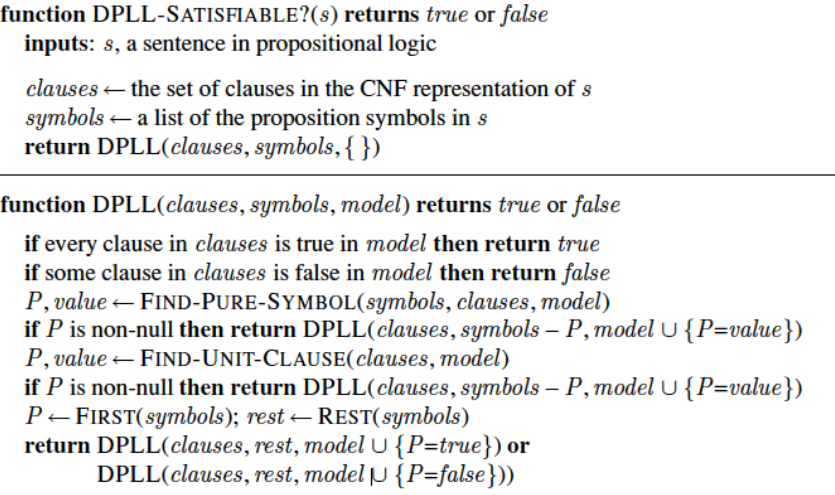
\includegraphics[width=\textwidth]{Images/dpll}
	\caption{Pseudocode of DPLL}
	\label{img:dpllPseudo}
\end{figure}

Walk-SAT is one (of many) local search methods and is to be used for SAT problems
where solutions exist and are evenly distributed; it is not complete and is 
very effective for large problems.

In figure \ref{img:walkSat} is possible to note the pseudocode to compute Walk-Sat and 
in figure \ref{img:comparisonDPLL} is possible to see a comparison between DPLL and WalkSat.

\begin{figure}
	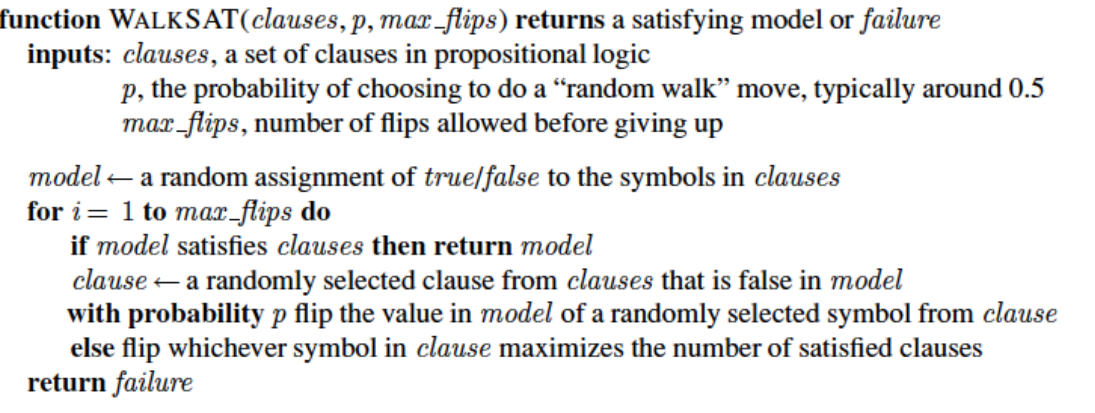
\includegraphics[width=\textwidth]{Images/walksat}
	\caption{Pseudocode of WalkSat}
	\label{img:walkSat}
\end{figure}

\begin{figure}
	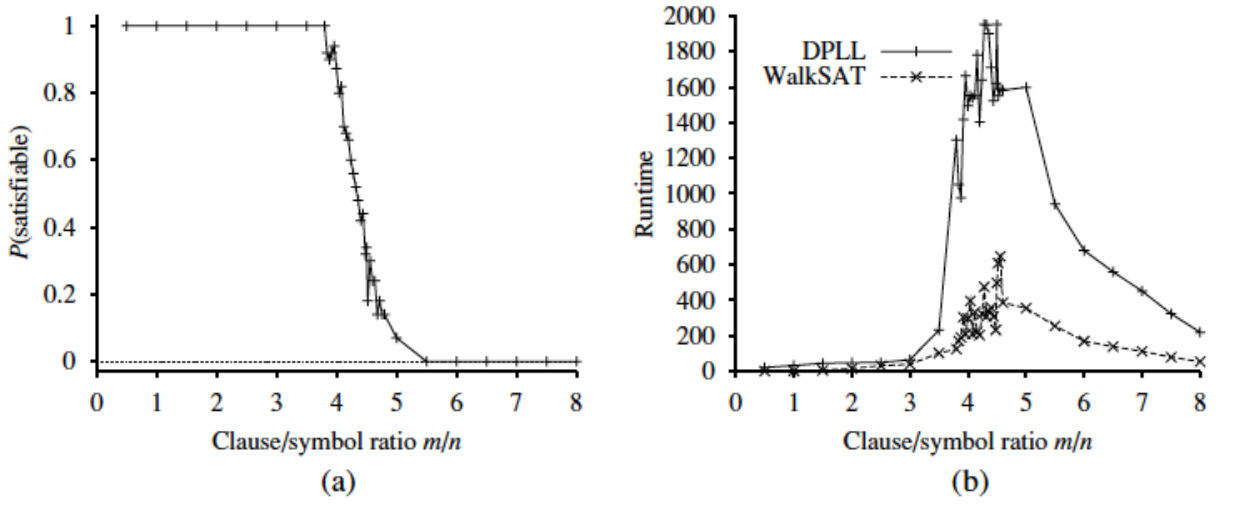
\includegraphics[width=\textwidth]{Images/dpllComparison}
	\caption{Comparison between DPLL and WalkSat}
	\label{img:comparisonDPLL}
\end{figure}
Also in the case of FOL you can obtain a clausal form in an effective way, and the 
transformation involves the elimination of existential quantifiers by Skolemization, so
\[ \exists x father(x, G) \text{ becomes } father(k, G) \]
This transformation preserves satisfiability, but not equivalence.

Given the fundamental problem $KB \models \alpha$ an equivalent problem is
$KB \cup \neg \alpha$ is unsatisfiable and this can be solved by a deductive system
showing that $KB \cup \neg \alpha \vdash \{ \}$, where $\{ \}$ is the
empty clause meaning False.

Resolution by refutation is a method which is correct and complete:
\begin{enumerate}
   \item transform the KB in clausal form (a conjunction of disjunction of literals)
   \item add to KB the negation of the goal in clausal form
   \item use the resolution rule as unique inference rule.
\end{enumerate}
This strategy works for PROP and FOL with different complexity results:
it is decidable and NP-complete for PROP, instead is semi-decidable for FOL.

Clauses are set of literals, so the resolution rule for PROP is the following
\[ \frac{c_1 \cup \{p\} \, \, \, \, c_2 \cup \{\neg p\}} {c_1 \cup c_2} \]
In a resolution refutation we aim to deduce the empty clause and the resolution rule
for FOL is the following:
\[ \frac{c_1 \cup \{ p \} \, \, \, \, c_2 \cup \{\neg q\}} {[c_1 \cup c_2]\gamma} \]
and $\gamma = MGU(p, q)$ and $\gamma$ is not fail, so a fundamental operation is 
\emph{unification}, who is a process to determine whether two expressions can be made
identical by a substitution of terms to variables, so 
the result is the unifying substitution, the unifier, or FAIL,
if the expressions are not unifiable.

Given two expressions there may be different substitutions that make them identical and 
we are interested in computing the most general unifier (MGU), the one that does only
the essential instantiations.

We present now the Unification algorithm, invented in $1982$ by Martelli and Montanari,
which consist in the following passes:
\begin{enumerate}
   \item Computes the MGU by means of a rule-based equation-rewriting system
   \item Initially the working memory (WM) contains the equality of the two
         expressions to be unified.
   \item The rules modify equations in the WM
   \item The algorithm terminates with failure or when there are no applicable rules
	 (success)
   \item At the end, if there is no failure, the WM contains the MGU.
\end{enumerate}
The rules used to compute the MGU are the following:
\begin{enumerate}
   \item $f(s_1, \dots, s_n) = f(t_1, \dots, t_n) \to s_1 =  t_1 , \dots, s_n = t_n$
   \item $f(s_1, \dots, s_n) = g(t_1, \dots, t_m) \to fail$ when $f \neq g$ or $n \neq m$.
   \item $x = x$ we can remove the equation
   \item $t = x \to x = t$ 
   \item $x = t, x$ does not occur in $t$ the nwe apply $\{x/t\}$ to other equations.
   \item $x = t, t$ is not $x$, $x$ occur in $t$ then we have fail.
\end{enumerate}
Note that when we compare two different constants, rule 2 applies, as a special case
where $n = m = 0$, and we fail.

\section{Knowledge \& Ontological Engineering}
\emph{Knowledge engineering} is the activity to formalize a specific problem or
task domain and it involves decisions about what are the relevant fact, objects and so on,
but also which is the right level of abstaction.\newline
\emph{Ontology engineering} seeks to build general-purpose ontologies which should be
applicable in any special-purpose domain (with the addition of domain-specific axioms). 

Before implementing, need to understand clearly, like in software engineering
what is to be computed, what kind of knowledge, why and where inference is necessary.

Sometimes useful to reduce n-ary predicates to 1-place predicates and 1-place functions,
that involves creating new individuals and new functions for properties/roles,
this is typical of description logics/frame languages, which we will talking later.

The use of KR languages and logic in A.I. is representing “common sense”
knowledge about the world, rather than mathematics or properties of programs.\newline
Common sense knowledge is difficult since it comes in different varieties and it
requires formalisms able to represent actions, events, time, physical objects, beliefs,
categories that occur in many different domains.

In figure \ref{img:general} is possible to note that a general ontology organizes 
everything in the world into a hierarchy of categories and should be applicable
in any special-purpose domain (with the addition of domain-specific axioms).\newline
In any non trivial domain, different areas of knowledge must be combined,
because reasoning and problem solving could involve several areas simultaneously and 
it is difficult to construct one best ontology, infact "Every ontology is a treaty—a
social agreement—among people with some common interest in sharing.”

\begin{figure}
	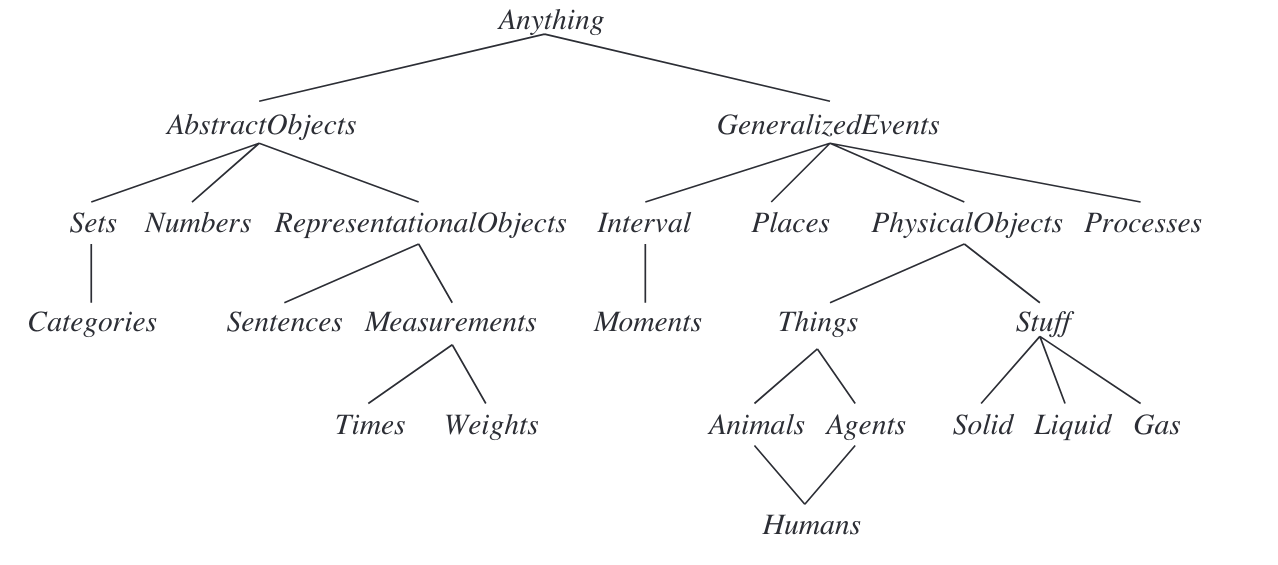
\includegraphics[width=\textwidth]{Images/generalOntology}
	\caption{General Ontology specification}
	\label{img:general}
\end{figure}
Much reasoning takes place at the level of categories, so we can infer category
membership from the perceived properties of an object, and then uses category
information to derive specific properties of the object.\newline
There are two choices for representing categories in first-order logic:
\begin{enumerate}
    \item Predicates, categories are unary predicates, that we assert of individuals:
    \item Objects: categories are objects that we talk about (\emph{reification}),
	  so for example the predicate $WinterSport(Ski)$ become $Ski \in WinterSports$
\end{enumerate}
In this way we can organize categories in taxonomies (like in natural sciences),
define disjoint categories, partitions and use specialized inference mechanisms,
such as inheritance. 

We use the general PartOf relation to say that one thing is part of another,
composite objects can be seen as part-of hierarchies, similar to the Subset hierarchy
and these are called \emph{mereological hierarchies}.

Composite objects is a structural relations among parts so 
for example, a biped has two legs attached to a body will be represented as a relation
among biped and leg.

\emph{Bunch} is a composite objects with definite parts but no particular structure,
so "a bag of three apples" will be represented by BunchOf($\{Apple_1, Apple_2, Apple_3\})$
that should not be confused with the set of $3$ apples and unlike sets, bunches have
weight; also we have that each element of category $s$ is part of BunchOf(s) and also
BunchOf(s) is the smallest object satisfying this condition (logical minimization).

Physical objects have height, weight, mass, cost, and so on and the values that we
assign for these properties are called measures.\newline
A solution is to represent measures with units functions that take a number as argument
so for example we have Length($L_1$) = Inches($1.5$) = Centimeters($3.81$).\newline
The most important aspect of measures is not the particular numerical
values/scale, but the fact that measures can be ordered, and to perform some sort
of qualitative inference, often it is enough to be able to order values 
and to compare quantities (qualitative physics).

There are countable objects, things such as apples, holes, and theorems, and
mass objects, such as butter, water, and energy, these are called Stuff.\newline
The properties of stuff are the following:
\begin{enumerate}
  \item Any part of butter is still butter, so we have in symbols
	\[ b \in  Butter \cap PartOf(p, b) \Rightarrow  p \in  Butter \]
  \item Stuff has a number of intrinsic properties (color, high-fat content, density \dots        ), shared by all its subparts, but no extrinsic properties, so it is a substance.
\end{enumerate}

\section{Situation Calculus}
The situation calculus is a specific ontology in FOL dealing with actions and change,
with the following concepts:
\begin{description}
    \item [Situations: ] snapshots of the world at a given instant of time,
	                 the result of an action.
    \item [Fluents: ]    time dependent properties.
    \item [Actions: ]    performed by an agent, but also events.
    \item [Change: ]     how the world changes as a result of actions.
\end{description}
We define Result as the effect of a sequence of actions, defined as a function
\[ Result: [A*] \times S \to S \]
with Result([], s) = s and Result([a | seq], s) = Result(seq, Result(a, s)).

The frame problem is one the most classical A.I. problems and the name comes from 
an analogy with the animation world, where the problem is to distinguish background
(the fixed part) from the foreground (things that change) from one frame to the other.
Let’s try to fix the problem writing frame axioms, such that an action remains true
unless someone makes false, but with frame axioms we have too many axioms
(representational frame problem).

We can combine preconditions, effect and frame axioms to obtain a more compact 
representation for each fluent $f$ and the schema is as follows:
$f$ true after true preconditions and some action made $f$ true or
f was true before and no action made it false.

The representational frame problem is considered to be (more or less) solved with 
this new definition and we have another problem, called \emph{Qualification problem},
since in real situations it is almost impossible to list
all the necessary and relevant preconditions.\newline
\emph{Ramification problem} is the problem of among derived propertied which ones
persist and which ones change?

What we would need is the ability to formalize a notion of persistence, that estabilish
that “in the absence of information to the contrary (by default)
things remain as they were”.\newline
Unfortunately this leads out of classical logic and the closure assumption we used 
is already an ad hoc form of completion and we will see more
of this strategy in nonmonotonic reasoning.\newline
In planning we end up using other languages that make stronger assumptions
and are more limited in their expressivity.

Situation calculus is limited in its applicability: Single agent, Actions are discrete
and instantaneous (no duration in time), Actions happen one at a time: no concurrency,
no simultaneous actions and only primitive actions, so there is no way 
to combine actions (conditionals, iterations and so on).\newline
To handle such cases we introduce an alternative formalism/ontology known as
\emph{event calculus}, which is based on events, points in time,
intervals rather than situations.

\section{Event Calculus}
Event calculus reifies fluents and events and the fluent is an object 
(represented by a function), so to assert that a fluent is true at some point
in time t we use the predicate T, so for example 
T(At(Shankar, Berkeley), t).

Events are described as instances of \emph{event categories}, so for example
the event $E_1$ of Shankar flying from San Francisco to Washington, D.C. is described as
\[ E_1 \in Flyings \cap Flyer(E_1 , Shankar) \cap Origin(E_1 , SF ) \cap 
   Destination(E_1 , DC) \]
By reifying events we make it possible to add any amount of arbitrary information
about them, such participants in the event or properties.

Time intervals are a pair of times $(start, end)$, so $i = (t_1, t_2)$
is the time interval that starts at $t_1$ and ends at $t_2$.\newline
We have the event Happens($E_1, i)$ to say that the event $E_1$ took place 
over the time interval $i$.\newline
The complete set of predicates for one version of the event calculus is the following:
\begin{description}
    \item [$T(f, t)$] fluent $f$ is true at time $t$.
    \item [Happens(e, i)] event $e$ happens over the time interval $i$.
    \item [Initiates(e, f, t)] event $e$ causes fluent $f$ to start at time $t$.
    \item [Terminates(e, f, t)] event $e$ causes fluent $f$ to cease at time $t$.
    \item [Clipped(f, i)] fluent $f$ ceases to be true at some point during 
	                  time interval $i$.
    \item [Restored(f, i)] fluent $f$ becomes true sometime during time interval $i$.
\end{description}
A fluent holds at a point in time if the fluent was initiated by an event at some
time in the past and was not made false (clipped) by an intervening event, so formally
\[ Happens(e, (t_1, t_2)) \cap Initiates(e, f, t_1) \cap \not Clipped(f, (t_1, t)) \cap
   t_1 < t \Rightarrow T(f, t) \]
A fluent does not hold at a point in time if the fluent was terminated by an event
at some time in the past and was not restored by an event occurring at a later time,
so formally we have
\[ Happens(e, (t_1, t_2)) \cap Terminates(e, f, t_1) \cap \not Restored(f, (t_1, t)) \cap
   t_1 < t \Rightarrow \not T(f, t) \]
where Clipped and Restored are defined by
\begin{align*}
	Clipped(f , (t_1 , t_2)) & \iff \exists e, t, t_3 Happens(e, (t, t_3)) \cap
	t_1 \leq t < t_2 \cap Terminates(e, f, t) \\
        Restored(f, (t_1, t_2)) & \iff \exists e, t, t_3 Happens(e , (t, t_3)) \cap
	t_1 \leq t < t_2 \cap Initiates(e, f, t) \\
\end{align*}
We can extend the predicate $T$ to hold over intervals, so we says that a fluent
holds over an interval if it is true at every point within the interval
\[ T(f, (t_1, t_2)) \iff [\forall t \, (t_1 \leq t < t_2) \Rightarrow T(f, t)] \]
Actions are modeled as events, and we have that fluents and actions are related
with domain-specific axioms that are similar to successor-state axioms.\newline
We can extend event calculus to make it possible to represent simultaneous
events, continuous events and so on.

\emph{Processes} or liquid events are events with the property that if they happen
over an interval also happen over any subinterval
\[ (e \in Processes) \cap Happens(e, (t_1, t_4)) \cap (t_1 < t_2 < t_3 < t_4)
   \Rightarrow Happens(e, (t_2, t_3)) \]
The distinction between liquid and nonliquid events is analogous to the
difference between substances, or stuff, and individual objects, or things.

We can model in detail the behavior of intervals, providing more vocabulary:
\begin{description}
   \item [Time(x)] points in a time scale, giving us absolute times in seconds.
   \item [Begin(i)] earliest moment in an interval.
   \item [End(i)] latest moment in an interval.
   \item [Duration(i)] the duration of an interval.
\end{description}
The Complete set of interval relations, proposed by Allen (1983) and visible in figure
\ref{img:timeInterval}, are the following:
\begin{itemize}
   \item $Meet(i, j) \iff End(i) = Begin(j)$
   \item $Before(i, j) \iff End(i) < Begin(j)$
   \item $After(j, i) \iff Before(i, j)$
   \item $During(i, j) \iff Begin(j) < Begin(i) < End(i) < End(j)$
   \item $Overlap(i, j) \iff Begin(i) < Begin(j) < End(i) < End(j)$
   \item $Begins(i, j) \iff Begin(i) = Begin(j)$
   \item $Finishes(i, j) \iff End(i) = End(j)$
   \item $Equals(i, j) \iff Begin(i) = Begin(j) \cap End(i) = End(j)$
\end{itemize}

\begin{figure}
	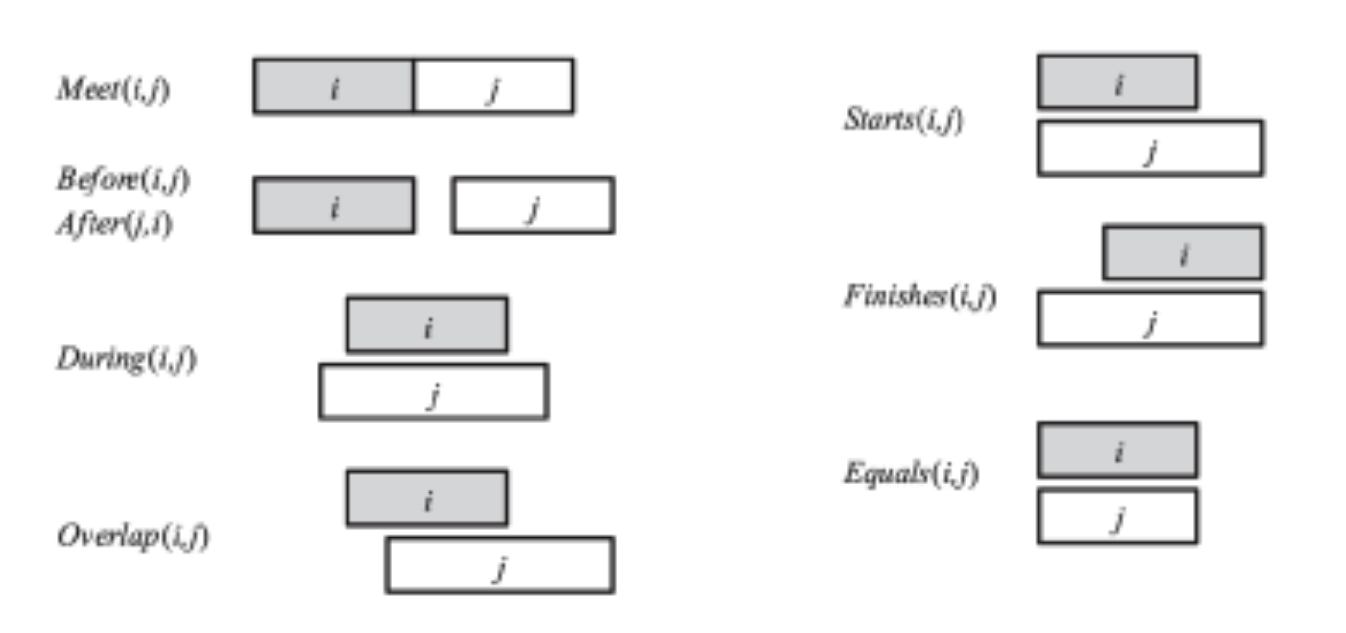
\includegraphics[width=\textwidth]{Images/intervalRelations}
	\caption{Visual representation of interval relations}
	\label{img:timeInterval}
\end{figure}

\section{Nonmonotonic reasoning}
Failures of monotonicity are widespread in commonsense reasoning, infact it seems
that humans often “jump to conclusions”, when they think it is safe to do so
(lacking information to the contrary).\newline
These conclusions are only “reasonable”, given what you know, rather than
classically entailed and also most of the inference we do is defeasible:
additional information, may lead to to retract those tentative conclusions.\newline
Any time the set of beliefs does not grow monotonically as new evidence arrives,
the monotonicity property is violated and including defeasible reasoning
leads us to consider nonsound inferences.

Some common instances of nonmonotonic reasoning are the following:
\begin{description}
   \item [Default reasoning: ] reasonable assumptions unless evidence of the contrary
   \item [Persistence: ] things stay the same, according to a principle of inertia,
	                 unless we know they change.
   \item [Economy of representation: ] only true facts are stored, false facts are only
                                       assumed.
   \item [Reasoning about knowledge:] if you have $\neg Know(p)$ and you learn $p$ we
	                              have $Know(p)$.
   \item [Abductive reasoning: ] most likely explanations to known facts.
\end{description}
Universal rules, like $\forall x (P(x) \Rightarrow Q(x))$, express properties that
apply to all instances, but most of what we learn about the world is 
in terms of generics rather than universals.\newline
Listing exceptions to generic properties is not a viable solution, so the goal is to 
be able to say a $P$ is a $Q$ in general, normally, but not necessarily.\newline
In this way it is reasonable to conclude $Q(a)$, given $P(a)$, 
unless there is a good reason not to and this is what we call a \emph{default}
and \emph{default reasoning} the tentative conclusion.

There are three ways to approach the problem, that we will analyze:
\begin{description}
   \item [Model theoretic formalizations (CWA, Circumscription):]
         consist in a restriction to the possible interpretations, 
         redefining the notion of entailment and we can still have systems
	 sound and complete wrt the new semantics.
   \item [Proof theoretic formalizations (Default logic, Autoepistemic logic):]
      A proof system with non-monotonic inference rules and autoepistemic logic
	(under the heading “logics for knowledge and beliefs”).
   \item [Systems supporting belief revision TMS, ATMS]
\end{description}
Under Closed World Assumption (CWA) only positive facts are stored, any other 
basic fact is assumed false and CWA assumption is used in [deductive] databases
and in logic programming with negation as failure.

CWA corresponds to a new version of entailment ($\models_c$) defined as 
\begin{defi}[CWA]
    $KB \models_c a$ if and only if $CWA(KB) \models a$ where 
    \[ CWA(KB) = KB \cup \{ \neg  p : \text{ p ground atom and } KB \not \models p \} \]
\end{defi}
$CWA(KB)$ is the completion under CWA of KB and note that the $CWA$ is nonmonotonic.

KB with consistent knowledge (satisfiable) happens when for no $\alpha \, KB \models \alpha$
and $KB \models \neg \alpha$, but normally a KB has incomplete knowledge.\newline
CWA can be seen as an assumption about complete knowledge, or a way to 
make a theory complete, using the following theorem:
\begin{thm}
    For every $\alpha$ (without quantifiers), $KB \models_c \alpha$ or 
$KB \models_c \neg \alpha$.
\end{thm}
$CWA(KB)$ is not always consistent when KB is consistent, infact there are problem
with disjunctions, so a solution is to restrict $CWA$ to atoms that are 
“uncontroversial”; CWA limited in such a way is called Generalized CWA (GCWA) and
is a weaker form of completion than unrestricted CWA (the assumed beliefs are less).
\begin{thm}[Consistency of CWA]
   $CWA(KB)$ is consistent iff whenever $KB \models (q_1 \vee \dots \vee q_n)$
   then $KB \models q_i$ for some $q_i$.\newline
   GCWA comes if $KB \models \{ p \vee q_1, \dots \vee q_n\}$ and $KB \not \models p$
   add $\neg p$ only if at least one ground literal $q_i$ is entailed.
\end{thm}
Since it may be difficult the condition of the theorem, the following corollary, which
restricts the application, is also of practical importance:
\begin{corol}
    If the clause form of $KB$ is Horn and consistent, then $CWA(KB)$ is consistent.
\end{corol}
The application of the theorem of consistency of $CWA$ depends on the terms 
that we allow as part of the language, and the Domain Closure Assumption (DCA) 
may be used to restrict the constants to those explicitly mentioned in the KB:
\[ \forall x. [x = c_1 \lor \dots \lor x = c_n] \]
where $c_i$ are all the finite constants appearing in KB.\newline
Under this restriction quantifiers can be replaced by finite conjunctions
and disjunctions and we also introduce the Unique Names assumption (UNA),
that can be used to deal with terms equality $c_i \neq c_j$ for $i \neq j$
but with functions things get more complicated.

With CWA we can reduce queries (without quantifiers) to atomic queries, by
repeated applications of the following properties:
\begin{enumerate}
    \item $KB \models_c (a \wedge b)$ iff $KB \models_c a$ and $KB \models_c b$
    \item $KB \models_c \neg \neg a$ iff $KB \models_c a$
    \item $KB \models_c \neg (a \vee b)$ iff 
	  $KB \models_c \neg a$ and $KB \models_c \neg b$
    \item $KB \models_c (a \vee b)$ iff $KB \models_c a$ or $KB \models_c b$
    \item $KB \models_c \neg(a \wedge b)$ iff
	  $KB \models_c \neg a$ or $KB \models_c \neg b$
\end{enumerate}
If $CWA(KB)$ is consistent, any query reduces to a set of atomic queries and we further
assume that $CWA(KB)$ is consistent we get
\[ KB \models_c \not a \iff KB \not \models_c a \] 
Much more efficient than ordinary logic reasoning (e.g. no reasoning by cases),
in fact we have restricted reasoning to a unique interpretation and instead of
checking validity/entailment we check truth in that interpretation.

In a \emph{vivid KB} we store this unique interpretation (a consistent and complete
set of literals) and answer questions retrieving from it, so a vivid KB
has the CWA builtin.\newline
If atoms are stored as a table, deciding if $KB \models_c \alpha$ is like DB-retrieval,
so instead of reasoning with sentences we reason about an analogical
representation of the world, or model.

The CWA is too strong for many applications, so we do not want to assume that any
ground atom not provable from the KB is false, because certain predicates
are considered complete, others are not.\newline
CWA wrt to a predicate P [set of predicates P]: the set of assumed beliefs is only
for ground atoms in P [predicates in P] and a similar theory is predicate completion
which consists in adding a set of completion axioms, so if only $P(A)$ and $P(B)$
are in KB we have that the completion axiom is defined as 
\[ \forall (x = a) \vee (x = b) \iff P(x) \]
The theory accounting for if and when this leads to consistent augmentation is
quite complex and a generalization of CWA and predicate completion is circumscription.

\emph{Circumscription} can be seen as a more powerful and precise version of the CWA,
working also for FOL, which was problematic and required further assumptions.\newline
The idea is to specify special abnormality predicates for dealing with exceptions and 
the definition of Circumscription is defined as 
\begin{defi}[Circumscription]
    Given the unary predicate Ab, consider only interpretations where $I[AB_f]$
    is as small as possible, relative to KB.
\end{defi}
Note that Circumscription is a semantic notion based on minimal models (a kind of
model preference logics) due to MacCarthy $1980$.

Let $P$ be a set of unary abnormality predicates and let $I_1$ and $I_2$ two 
interpretations that agree on the values of constants and functions so we define 
the ordering and minimal entailment as 
\begin{defi}[Minimal Entailment]
  $I_1 < I_2$ iff same domain and $\forall p \in P I_1[p] \subset I_2[p]$ holds and the 
  minimal entailment estabilish that $KB \models _{\leq} \alpha$ iff for every 
  interpretation $I$, if $I[KB] = T$ and such that there is no other interpretation $I'<I$
  such that $I'[KB] = T$ then $\alpha$ is true in $I$.
\end{defi}
In simpler words, $\alpha$ need not be true in all interpretations satisfying KB
but only in all those that minimize abnormalities (all the interpretations that
are most “normal”) and also that Circumscription need not produce
a unique minimal interpretation.

Although the default assumptions made by circumscription are usually weaker than
those of the CWA, there are cases where they appear too strong, so suppose for example,
that we have the following KB:
\begin{align*}
  \forall x [Bird(x) \wedge \not Ab(x) \Rightarrow Flies(x)] \\
  Bird(tweety) \\
  \forall x [Penguin(x) \Rightarrow (Bird(x) \wedge \not Flies(x))] \\
\end{align*}
From this follows that 
\[ \forall x [Penguin(x) \Rightarrow Ab(x)] \]
Minimizing abnormalities leads to $KB \models_{\leq} \not \exists x Ab(x)$ but also
$KB \models_{\leq} \not \exists x Penguin(x)$.

Partial fix is done using McCarthy's definition related to predicate completion, so
distinguish between P (variable predicates) and Q (fixed predicates).\newline
Ordering on interpretations is different for the two sets, so only predicates in $P$
are allowed to be minimized and $\forall Q \in \mathbf{Q} I_1[Q] = I_2[Q]$.

Default logic uses beliefs as deductive theory and uses $KB = <F, D>$ where 
$F$ is a set of sentences (facts) and $D$ is a set of default rules of type 
\[ \frac{\alpha : \beta}{\gamma} \]
Default rules where $\beta = \gamma$ are called \emph{normal defaults}.

Problem is now how to characterize theorems/entailments, because we cannot write a 
derivation, since do not know when to apply default rules and there is 
no guarantee of unique set of theorems, so we define \emph{extensions} as
sets of sentences that are "reasonable" beliefs, given explicit facts and 
default rules.

$E$ is an extension of $<F, D>$ iff for every sentence $\pi, E$ satisfies the 
following $\pi \in E \iff F \cup \Delta \models \pi$, where 
\[ \Delta = \{ \gamma : \frac{\alpha : \beta}{\gamma} \in D, \alpha \in E, 
                        \not \beta \not \in E\} \]
So, an extension $E$ is the set of entailments of $F \cup \Delta$ , where the
$\Delta$ are a “suitable” set of assumptions given $D$.\newline
Note that $\alpha$ has to be in $E$ , not in $F$ and this has the effect of allowing
the prerequisite to be believed as the result of other default assumptions.

If E is inconsistent we can conclude anything we want, so we have this theorem
\begin{thm}
   An extension of a default theory is inconsistent iff the original $F$ is inconsistent.
\end{thm}
In this case the extension is unique, but in general a default theory
can have multiple extensions.

The properties of Default logics are the following:
\begin{enumerate}
    \item If a default theory has distinct extensions, they are mutually inconsistent.
    \item There are default theories with no extensions.
    \item Any normal default theory has an extension.
    \item Adding new normal default rules does not require the withdrawal of beliefs,
          even if adding new beliefs might, some normal default theories 
	  are semi-nonmonotonic.
\end{enumerate}
We have a problem that leads to a more complex definition of extension, so suppose 
$F = \{ \}$ and $D = \{: p / p\}$ then $E = $ entailments of $\{p\}$ is an extension
since $p \in E$ and $\not p \not \in E$.\newline
However, we have no good reason to believe p, since only support for $p$ is the
default rule, which requires $p$ itself as a prerequisite, so the default should
have no effect; for this reason we define a revision of definition of extension with
\begin{defi}[Grounded extension]
    For any set $S$, let $\Gamma(S)$ be the least set containing $F$, closed under 
    entailment, and satisfying 
    \[ \alpha: \beta / \gamma \in D, \alpha \in \Gamma(S), \not \beta \not \in S 
	\Rightarrow \gamma \in \Gamma(S) \]
\end{defi}
A set $E$ is an extension of <$F, D$> iff $E = \Gamma(E)$, so $E$ is a fixed point
of the $\Gamma$ operator.

\section{Knowledge and beliefs}
Human intelligence is intrinsically social, since humans need to negotiate and
coordinate with other agents, so in multi-agent scenarios, we need methods for
one agent to model mental states of other agents: high level representations of
other agent’s belief, intentions and goals may be relevant for acting;
by mental states we mean the relation of an agent to a proposition and 
propositional attitudes that an agent can have include Believes, Knows, Wants,
Intends, Desires, Informs, so called because the argument is a proposition, and 
also propositional attitudes do not behave as regular predicates.

A property important is called \emph{referential transparency}, which means that 
what matters is the object that the term names, not the form of the term, but 
propositional attitudes like Believes and knows, require referential opacity, 
the terms used do matter, because an agent may not be aware
of which terms are co-referential.

To implement knowledge and beliefs there are three approaches:
\begin{description}
   \item [Reitification: ] we remain within FOL, as we did for the situation calculus,
	   using terms to represent propositions, so for example $Bel(a, On(b, c))$,
	   but suffer for Referential transparency problem.
   \item [Meta-linguistic representation: ] we remain within FOL and represent
	   propositions as strings, so for example Bel(a, "On(b, c)").
   \item [Modal logics: ] propositional attitudes are represented as modal operators
	   in specialized modal logics, with alternative semantics and modal operators
	   are an extension of classical logical operators, so for example we have
	   B(a, On(b, c)) or $B_A$(On(b, c)) to say that agent a believes($B$)/
	   knows($K$) that block $B$ is on $C$.
\end{description}
Classical logic has only one modality (the modality of truth), so $P$ is the same as 
saying "$P$ is true".

Strictly speaking modal logic is about necessity and possibility, however, the
term is used more broadly to cover logics with different modelling goals.
$\square A$ means that it is necessary that $A$ instead $\diamond A$ means that 
it is possible that $A$, and these two operators are related, as $\exists$ and $\forall$
in First Order logic.

The simplest logic is called $K$ (after Saul Kripke), that results from adding the
following to the principles of propositional logic:
\begin{description}
    \item [Necessitation Rule:] if $A$ is a theorem of $K$, then so is $\square A$.
    \item [Distribution Axiom: ] $\square (A \Rightarrow B) \Rightarrow 
	                          (\square A \Rightarrow \square B)$
\end{description}
$\square$ is some sort of universal quantification over interpretations and 
$\diamond$ is some sort of existential quantification over interpretations.

Logic $T$ adds axiom $\square A \Rightarrow A$, that may be relevant for some
modal operators and not for others, so for example Knows $A \Rightarrow A$ seems plausible
instead Bel $A \Rightarrow A$ is not.\newline
Logic $S4$ adds $\square A \Rightarrow \square \square A$ and logic $S5$ adds
$\diamond A \Rightarrow \square \diamond A$.

Semantics for modal logics is defined by introducing a set $W$ of possible worlds
and an accessibility relation $R$ between worlds, so the interpretation of a formula
is now with respect to a possible world $w$ and we write $I(A, w)$.\newline
The interpretation formula for operators from classic logic are the same instead 
the interpretation formula for $\square$ and $\diamond$ are the following
\begin{align*}
    I(\square A, w) = T & \text{ iff for every world } w' \in W \text{ such that } wRw'
                          I(A, w') = T \\
    I(\diamond A, w) = T & \text{ iff for some world} w' \in W \text{ such that} 
	                        wRw' I(A, w') T \\
\end{align*}
Different modal logics are defined according to the properties of the accessibility
relation R (and corresponding axioms).

Modal logics address the problem of referential transparency, since the truth of a
complex formula does not depend on the truth of the components in the same
world/interpretation.\newline
Modal operators are not compositional, so the truth of Knows(A, P) cannot simply be
determined by the components of Knows , the denotation of the agent 
and the truth value of P.\newline
Modal logics for knowledge are easier than those of beliefs, so we start with these.

The syntax of modal logic for knowledge is the following:
\begin{enumerate}
   \item All the wff of ordinary FOL are also wff of the modal language.
   \item If $\Phi$ is a closed wff of the modal language and $a$ is an agent, 
	 then $K(a, \Phi)$ is a formula of the modal language.
   \item If $\Phi$ and $\Psi$ are wff so are the formulas that can be constructed
	 from them with the usual logic connectives.
\end{enumerate}
Examples of Formulas are the following:
\[ K(A_1, K(A_2 , On(B, C)) \]
\[ K(A_1, On(B, C)) \lor K(A_1 , \not On(B, C)) \]
\[ \not K(A_1, On(B, C )) \]
Properties of knowledge which are desirable to have are:
\begin{itemize}
 \item One agent can hold false beliefs but cannot hold false knowledge and if an agent
       knows something than this must be true, so knowledge is justified by true belief.
 \item An agent does not know all the truths: something may be true without the agent
       knowing it.
 \item If two formulas $\Phi$ and $\Psi$ are equivalent not necessarily $K(A, \Psi)$
       implies $K(A , \Psi)$
\end{itemize}
The semantics of modal logic is given in terms of possible worlds and specific
accessibility relations among them, one for each agent.\newline
An agent knows a proposition just when that proposition is true in all the worlds
accessible from the agent’s world (those that the agent considers possible).

Possible worlds roughly correspond to interpretations and an accessibility relation
($k$ for knowledge) is defined between agents and possible worlds:
\begin{defi}[Accessibility Relation]
	If $k(a, w_i, w_j)$ is satisfied, then world $w_j$ is accessible from 
	world $w_i$ for agent $a$.
\end{defi}
The semantic of Modal logic for knowledge is defined with the following rules:
\begin{enumerate}
  \item Regular wffs (with no modal operators) are not simply true or false but
	they are true or false wrt a possible world, so $I(w_1, \Phi)$ may be 
        different from $I(w_2, \Psi)$.
  \item A modal formula $K(a, \Psi)$ is true in $w$ iff $\Psi$ is true in all the worlds
	accessible from $w$ for agent $a$.
  \item The semantics of complex formulas is determined by regular truth recursive rules.
\end{enumerate}
$K(A, \Psi)$ means that agent $A$ knows the proposition denoted by $\Psi$ and 
"Not knowing $\Psi$" in $w_0$ (a specific world) is modelled by allowing worlds,
accessible from $w_0$, in which $\Psi$ is true and some worlds in which $\Psi$ is false.

The accessibility relation also accounts for nested knowledge statements and 
involving different agents, so as we can see in figure \ref{img:nestedKnowledge},
$K(A, K(B, P))$ holds in $w_0$ since $K(B, P)$ holds in $w_0, w_1, w_2$ and $w_3$.

\begin{figure}
    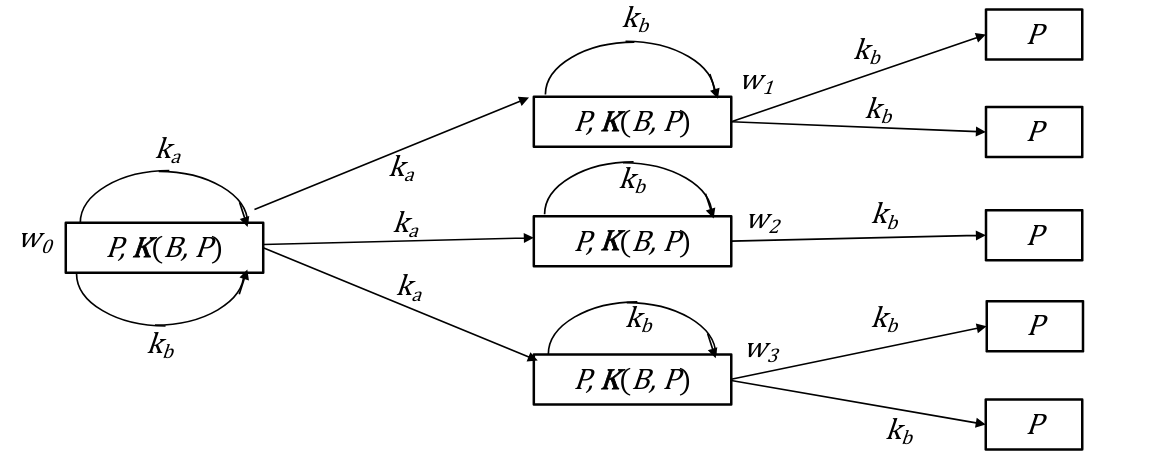
\includegraphics[width=\textwidth]{Images/nestedKnowledge}
    \caption{Example of Nested knowledge statements}
    \label{img:nestedKnowledge}
\end{figure}
Many of the properties that we desire for knowledge (and belief) can be achieved by
imposing constraints to the accessibility relation, so we define:
\begin{enumerate}
   \item Agents should be able to reason with the knowledge they have
         \[ K(a , \alpha \Rightarrow \beta) \Rightarrow (K(a, \alpha) \Rightarrow 
	    K(a, \beta)) \]
	 This is implicit in possible world semantics and is called 
	 \emph{Distribution axiom}.
   \item Agents cannot have false knowledge (different for beliefs)
         $K(a, \alpha) \Rightarrow  \alpha$ and this is called \emph{Knowledge axiom}.

	 The knowledge axiom is satisfied if the accessibility relation is reflexive and 
         this implies that there is at least a world accessible from $w$.

   \item It is also reasonable to assume that if an agent knows something, than it 
	 knows that it knows, that is formally
	 \[ K(a, \alpha) \Rightarrow K(a, K(a, \alpha)) \]
	 The accessibility relation must be transitive and this property is called
	 \emph{positive introspection}.
   \item In some axiomatization we also assume that if an agent doesn't know something,
         then it knows that it doesn't know it, that is formally
	 \[ \not K(a, \alpha) \Rightarrow K(a, \not K(a, \alpha)) \]
	The accessibility relation must be euclidean and this property is called
	\emph{Negative introspection}
   \item It is also intrinsic in possible world semantics that an agent knows all
	 the logical theorems, including the ones characterizing knowledge.\newline
         From $\vdash \alpha$ infer $K(a, \alpha)$ and this is 
	 \emph{Epistemic necessitation rule}.
   \item From 1 and 5, in the propositional case we also get rules
	 \[ \alpha \vdash \beta \land K(a, \alpha) \text{ we infer } K(a, \beta) \]
	 \[ \vdash \alpha \Rightarrow \beta \text{ we infer} 
	    K(a, \alpha) \Rightarrow K(a, \beta) \]
	 This is called \emph{Logical omniscience}, that is considered problematic,
	 since we are assuming unbounded reasoning capabilities.\newline
	As a corollary of logical omniscence we can infer $K$ distribution over and
	\[ K(a, \alpha \land \beta) \equiv K(a, \alpha) \land K(a, \beta) \]
\end{enumerate}

Modal epistemic logics are obtained with various combinations of axioms $1$-$4$ 
plus inference rule $5$, so we have System $K$ has only axiom $1$, system $T$ has 
axioms $1$-$2$, logic $S4$ has axioms $1$-$3$ and logic $S5$ has axioms $1$-$4$.\newline
Not any combination is possible since the properties of accessibility relations are
interdependent, so for example reflexive implies serial and if a relation is 
reflexive and Euclidian it is also transitive (axiom $2$ and $4$ imply $3$).

We have also consider the wise-men puzzle visible in figure \ref{img:wisemen}, where
we can also see an explanation of what consist.

\begin{figure}
	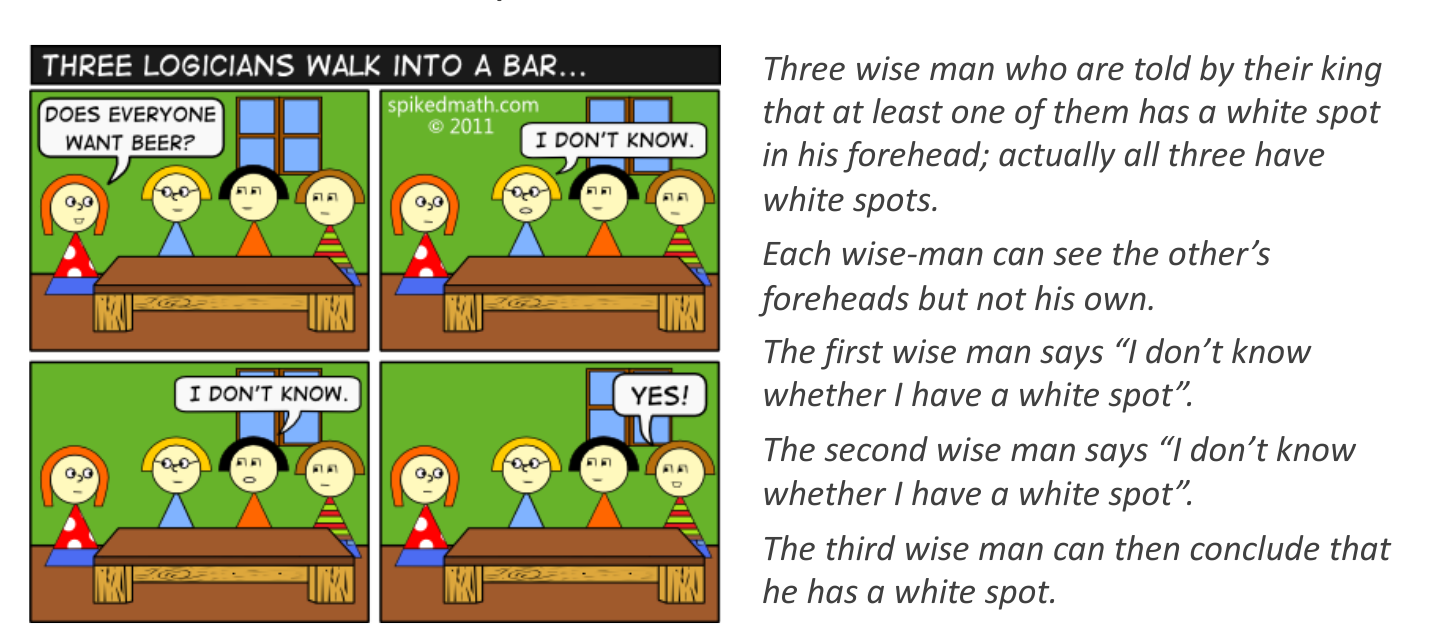
\includegraphics[width=0.8\textwidth]{Images/wiseman}
	\caption{Description of Wise-men puzzle}
	\label{img:wisemen}
\end{figure}
Since an agent can hold wrong beliefs the knowledge axiom is not appropriate, so 
we include as axiom the following instead
\[ \not B(a, False) \]
The distribution axiom and the necessitation rule are controversial, since an agent
cannot realistically believe all the logical consequences of its beliefs but
only those that he is able to derive (limited/bounded rationality), so 
\[ B(a, \alpha) \Rightarrow B(a, B(a, \alpha)) \]
\[ B(a, \alpha) \Rightarrow K(a, B(a, \alpha)) \]
Negative introspection is problematicm but with the following special case of
the knowledge axioms is safe $B(a, B(a, \alpha)) \Rightarrow B(a, \alpha)$

One disadvantage of default logic is that default rules are not sentences and
cannot be combined or reasoned about, so for example $\alpha: \beta / \gamma$
does not derive $\alpha: \beta / (\gamma \lor \delta)$.\newline
A different approach is to reason about defaults within a logic with a belief
operator $B$, where $B\alpha$ stands for "$\alpha$ is believed to be true”, and this
is \emph{autoepistemic logic}.\newline
The $B$ operator could be used to represent defaults, for example, as follows
\[ \forall x Bird(x) \land \not B \not Flies(x) \Rightarrow Flies(x) \]
Note that $B \not Flies(x)$ is different from $\not Flies(x)$

Given a KB that contains sentences using the B “auto-epistemic” operator, the 
minimal properties for a set of beliefs $E$ to be considered stable are the reasonable
set of beliefs to hold:
\begin{description}
 \item [Closure under entailment: ] if $E \models \alpha$, then $\alpha \in E$.
 \item [Positive introspection: ] if $\alpha \in E$, then $B \alpha \in E$.
 \item [Negative introspection: ] if $\alpha \not \in E$, then $\not B \alpha \in E$
\end{description}
This leads to the following definition of stable expansion of a KB
(a minimal set satisfying the properties yet described)
\begin{defi}[Stable expansion]
  A set $E$ is a stable expansion of $KB$ if and only if for every sentence $\phi$,
  it is the case that
  \[ \phi \in E \iff KB \cup \{B\alpha : \alpha \in E\} \cup 
                     \{\not B \alpha : \alpha \not \in E\} \models \phi \]
\end{defi}
The implicit beliefs $E$ are those sentences that are entailed by KB plus the 
assumptions deriving from positive and negative introspection.

The KB consisting of the sentence $(\not B p \Rightarrow p)$ has no stable expansion,
since if $B p$ is false, then the expansion entails $p$ and if $B p$ is true, then the
expansion does not include $p$.\newline
The KB consisting of the sentences $(\not B p \Rightarrow q)$ and $(\not B q \Rightarrow p)$
has exactly two stable expansions, so if $B p$ is true and $B q$ false the KB entails
$p$ and does not entail $q$, another stable expansion is when $B p$ is false and 
$B q$ is true.

\section{Reason Maintenance Systems}
Reason Maintenance Systems are the monotonic view of reasoning, so truth never changes,
the only allowed reasoning is to discover new truths.\newline
If the KB becomes inconsistent, there is not much you can do and common sense
reasoning requires belief revision mechanisms.\newline
We want to be able to make assumptions (defeasible reasoning) and if the world changes,
RETRACT is also an option (belief update).

RMS are practical systems designed to support beliefs revision, since they record
the reasons for believing something and do the job of maintaning consistency
in the belief set on behalf of the problem solver.

Many of the inferences drawn by a knowledge representation system will have only
default status or tentative nature and inevitably, some of these inferred facts
will have to be retracted; this process is called \emph{belief revision} and
can be problematic.\newline
One simple approach to belief revision is to number sentences according to the order
of assertion $P_1, P_2, \dots P_n$, so when the call $RETRACT(KB, P_i)$ is made, the 
system revert to the state just before $P_i$ was added, removing both $P_i$ and any
inferences derived from $P_i$.\newline
Sentences $P_{i+1}$ through $P_n$ can be added again if it is the case.

Reason Maintenance Systems (JTMS, ATMS), are reasoning mechanisms designed to handle
these problems efficiently and general architecture is visible in figure \ref{img:rms},
where the problem solver communicates facts, rules, assumptions along with their
justifications to the RMS and the PS may retract assertions, or may request to
handle inconsistencies.\newline
The RMS maintains beliefs, handles contradictions, restores consistency, performs
beliefs revision, generates explanations and provides the PS 
with an up-to-date set of beliefs.

\begin{figure}
	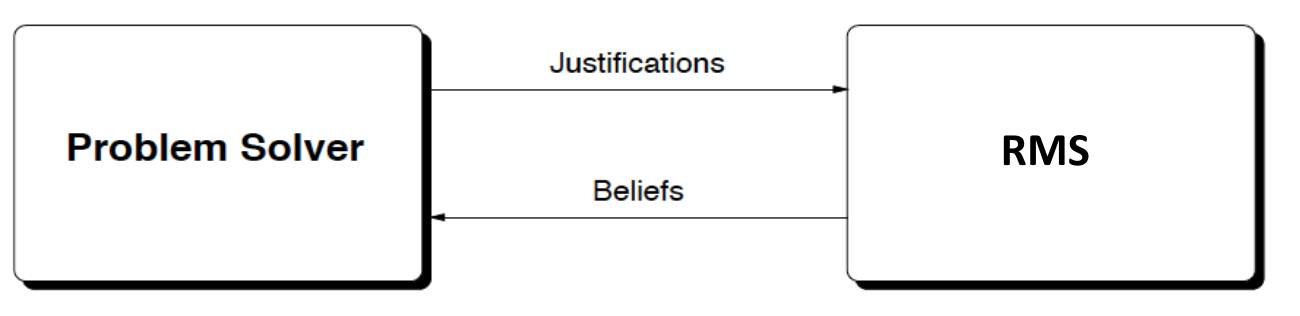
\includegraphics[width=\textwidth]{Images/architectureRMS}
	\caption{General Architecture of RMS}
	\label{img:rms}
\end{figure}
Rational thought is the process of finding reasons for attitudes, so has justified
belief or reasoned argument, rather than truth and the RMS handles a network of nodes
as propositional variables, representing propositions, rules and justifications.

Nodes are of different types: premises, assumptions, contradictions and have different
support according to the type of RMS and we will look at two of them:
\begin{itemize}
  \item JTMS (Justification-based Truth Maintenance Systems).
  \item ATMS (Assumption-based Truth Maintenance Systems)
\end{itemize}
In JTMS Each assertion in the knowledge base is represented as a node in the TMS with an
associated set of SL-justifications.\newline
Each SL-justification has two components:
\begin{description}
    \item [Inlist: ] the set of sentences from which it was inferred.
    \item [Outlist: ] a nonmonotonic justification the set of propositions that
	             should be false for the beliefs to be supported.
\end{description}
Examples:
\[ R (SL \{ \} \{ \}) \]
\[ Q (SL \{P, P \Rightarrow Q \}, \{\}) \]
\[ P (SL \{ \} \{\neg  P \}) \]
A node can have more than one SL justification (a justification set), since there
can be different reasons.

With JTMS, $RETRACT(KB, P)$ will delete exactly those sentences for which $P$ is a
member of every justification, so we have the following cases:
\begin{itemize}
 \item If a sentence $Q$ had the single justification $\{P, P \Rightarrow Q \}$, 
       then $Q$ would be removed.
 \item If it had the additional justification $\{P, P \lor R \Rightarrow Q \}$,
       then $Q$ would still be removed.
 \item If it also had the justification $\{R, P \lor R \Rightarrow Q \}$,
       then $Q$ would be maintained.
\end{itemize}
The JTMS, rather than deleting a sentence from the knowledge base
entirely when it loses all justifications, marks the sentence as being "out".\newline
If a subsequent assertion restores one of the justifications, then the
sentence is marked as "in" again, so we no need to re-compute inferences.

The node for proposition $P$ can be in one of two support states:
\begin{description}
 \item [IN: ] $P$ has at least one currently valid reason/justification,
	      and thus is a member of the current beliefs.
 \item [OUT: ] $P$ has no currently acceptable reason/justifications and
	       thus is not a member of the current beliefs.
\end{description}
A justification (SL inlist outlist) is valid iff each node in its inlist is IN,
and each node in its outlist is OUT and this creates a network of dependencies.\newline
Beliefs revision algorithms operate on these networks propagating effects and 
an example of that is visible in figure \ref{img:slList} and \ref{img:exSlList}.

\begin{figure}
	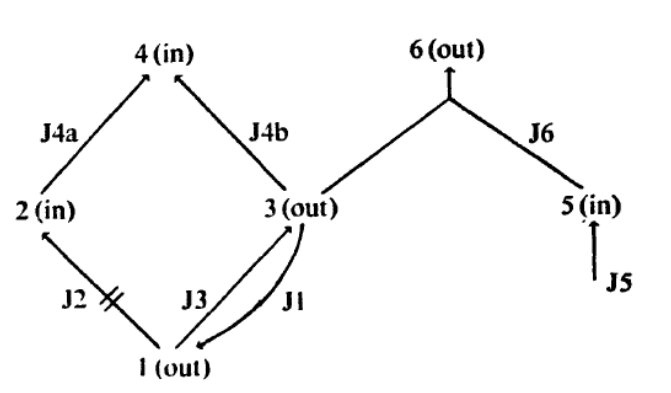
\includegraphics[width=\textwidth]{Images/slList}
	\caption{Example of SlList}
	\label{img:slList}
\end{figure}

\begin{figure}
	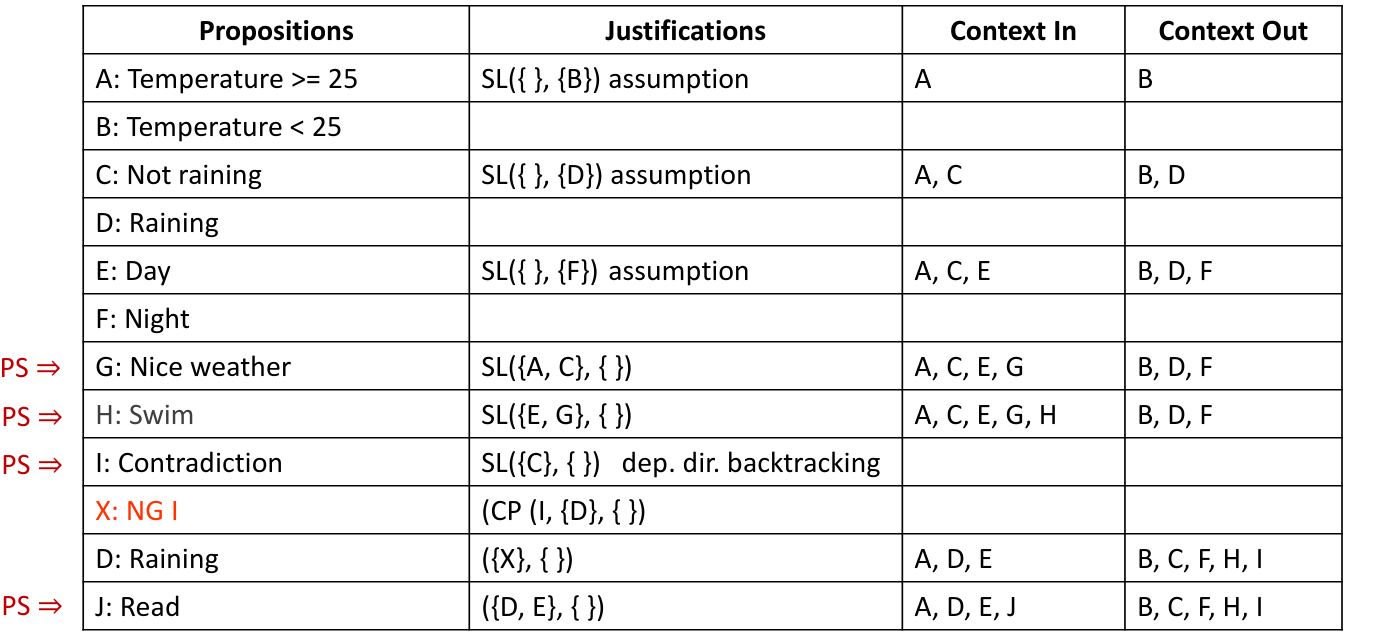
\includegraphics[width=\textwidth]{Images/exampleSlList}
	\caption{Complete example of Sllist in JTMS system}
	\label{img:exSlList}
\end{figure}

JTMSs can be used to speed up the analysis of multiple hypothetical situations, so
in a JTMS, the maintenance of justifications allows you to move quickly from one
state to another by making a few retractions and assertions, but at any time only
one contexts is represented.\newline
Taking the idea one step forward we could let multiple contexts to co-exist rather
than a global state of INs and OUT’s.

An Assumption based Truth Maintenance System (ATMS) represents all the contexts
been considered at the same time, so alternative contexts are explicitly stored.\newline
An ATMS-node is characterized by a label and justifications:
\begin{itemize}
 \item The label consists in a number of assumption sets (environments) and 
       the node holds when there is at least one supporting environment
       (with true assumptions).
 \item ATMS justifications are Horn formulas of the form $C :- L_1, L_2, \dots, L_n$,
       where $L_1, L_2, \dots, L_n$ are the antecendents and $C$ is the consequent of 
       justistification.
\end{itemize}
Thus a node is a triple $<n, E, J>$, where $n$ stands for an external sentence,
the description and in figure \ref{img:dependencyGraph} is possible to note an 
example of dependency graph.

\begin{figure}
	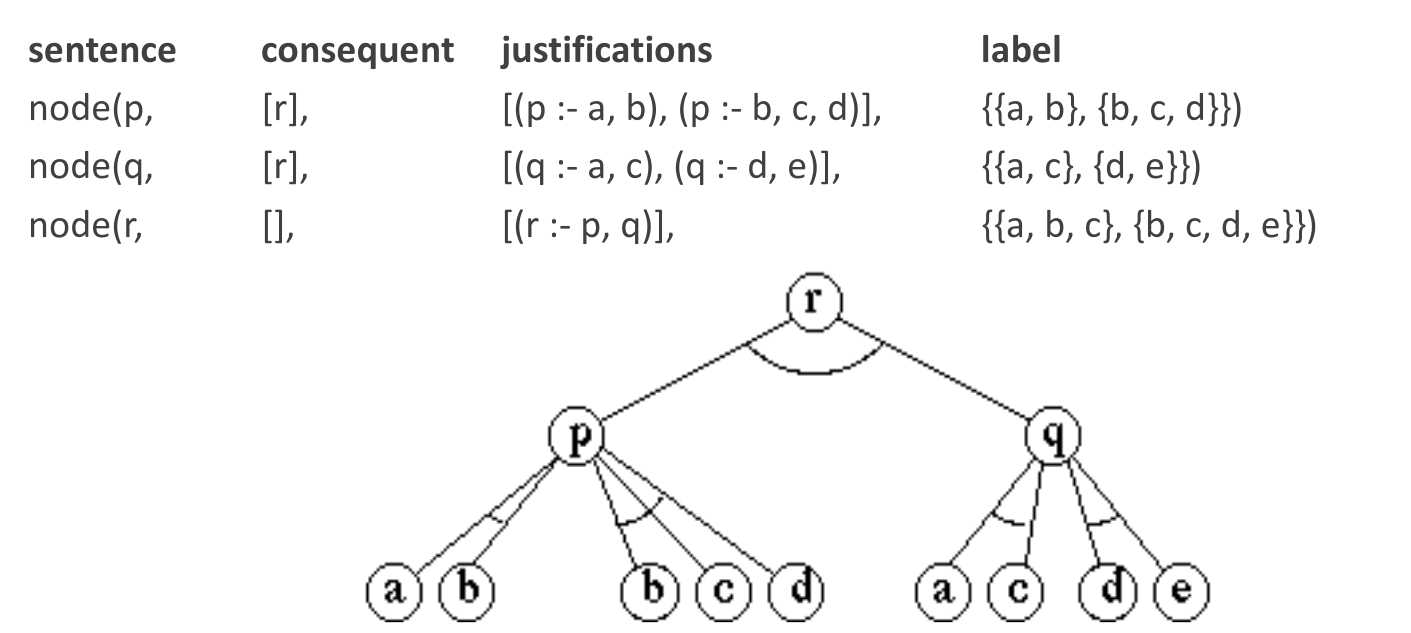
\includegraphics[width=\textwidth]{Images/dependencyGraph}
	\caption{Example of ATMS Dependency graph}
	\label{img:dependencyGraph}
\end{figure}

We have four types of nodes, according to the form of E and of J:
\begin{description}
 \item [Premise nodes: ] nodes always true, so the proposition can be believed
	                 without having to assume anything ($<n, \{\{ \}\}, \{( )\}>$.
 \item [Assumption nodes: ] these nodes are justified by themselves $<n, \{(n)\},\{(n)\}>$
 \item [Derived nodes: ] Maintain the set of assumptions made and the justifications.
 \item [Contradictions: ] an environment can be inconsistent when its assumptions are
	 contradictory, therefore must be removed, and these environments
	 are called \emph{nogoods}.
\end{description}
The fundamental operation is updating environments and deciding whether a
proposition holds in a given environment, so a node $n$ holds in a given 
environment $E$, iff it can be derived from $E$ given 
the set of justifications $J: E, J \vdash n$.

ATMS allow for quick generation of explanations, so an explanation of a sentence
$P$ is a set of sentences $E$ such that $E \models P$, usually a minimal
one is preferred and explanations can be assumptions.\newline
ATMS can generate explanations by making tentative assumptions and looking if the
label for the sentence  "car won’t start" contains the assumptions
that would justify the sentence.

\section{Semantic Networks and Frames}
We have that the logical approach is suitable to model rational reasoning, instead 
the cognitive–linguistic approach is more concerned with understanding the mechanisms
for knowledge acquisition, representation and use of knowledge in human minds and 
has synergies with other fields, such as cognitive psychology and linguistics.

In logic systems, symbolic expressions are modular and are syntactically transformed
without paying attention to the symbols used or to their “meaning”, infact 
the symbol themselves are arbitrary and it is all a matter of writing axioms 
to restrict interpretations.\newline
Associationist theories are instead concerned with the connections among symbols and
the meaning that emerges from these connections.\newline
The idea is that meaning of a word emerges as a result of the connections to other words
and connections are shaped by experience, as for example from reading texts.

The question is how the meaning of words is acquired, represented and used, and we have that
the memory itself is distinguished in:
\begin{description}
   \item [Episodic memory: ] specific facts and events.
   \item [Semantic memory: ] abstract and general knowledge.
\end{description}
Semantic networks is a graphical model proposed for semantic memory and we 
represent two kinds of knowledge:
\begin{description}
   \item [Concepts: ] the semantic counterpart of words, represented as nodes.
   \item [Propositions: ] relations among concepts, represented as labelled arcs.
\end{description}
It is not accounting for dynamic aspects of memory and learning and there are other models
like \emph{Distributional models}, like word embeddings,
or connectionist models for learning.

\begin{figure}
	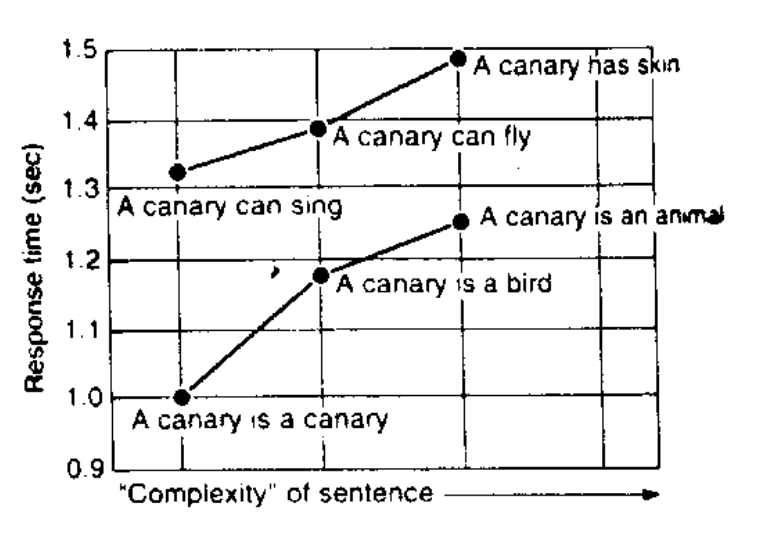
\includegraphics[width=\textwidth]{Images/cognitive}
	\caption{Example of a cognitive psychology definition}
	\label{img:cognitive}
\end{figure}

Cognitive psychology is an experimental discipline and
we have an example in figure \ref{img:cognitive}.\newline
Evidence are for hierarchical organization, properties are attached to the most general
concept to which they apply and exceptions are attached directly to the objects, like 
as possible to note in figure \ref{img:hierarchical}.\newline
Success of hierarchical organization of concepts in computer science and
influence on OOP languages in SW engineering.

\begin{figure}
	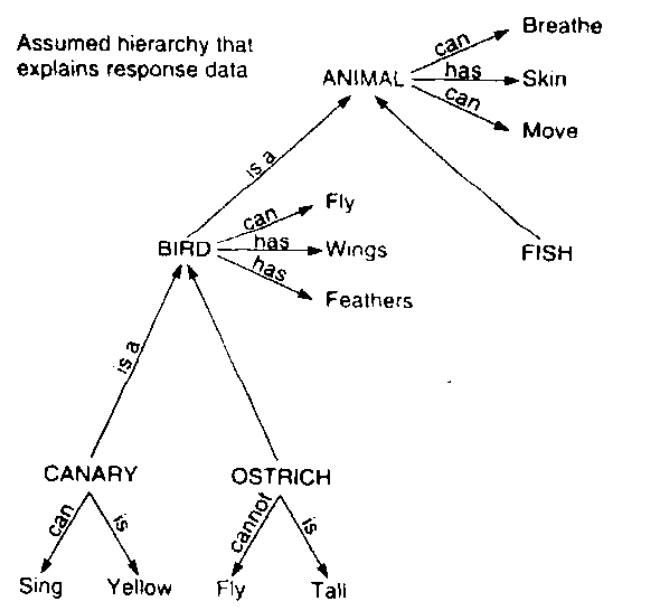
\includegraphics[width=\textwidth]{Images/hierarchical}
	\caption{Example of Hierarchical organization}
	\label{img:hierarchical}
\end{figure}

Semantic networks are a large family of graphical representation schemes and 
a semantic network is a graph where nodes, with a label, correspond to concepts
and arcs, labelled and directed, correspond to binary relations
between concepts, often called roles.\newline
Nodes come in two flavors:
\begin{description}
   \item [Generic concepts] corresponding to categories/classes
   \item [Individual concepts], corresponding to individuals
\end{description}
Two special relations are always present, with different names:
\begin{description}
    \item [IS-A: ]    holds between two generic concepts (subclass).
    \item [Inst-Of: ] holds between an individual concept and a class (member of).
\end{description}
Inheritance is very conveniently implemented as link traversal, as we can see in figure 
\ref{img:inheritance}, and Multiple inheritance is also allowed, but is banned in OOP.

\begin{figure}
	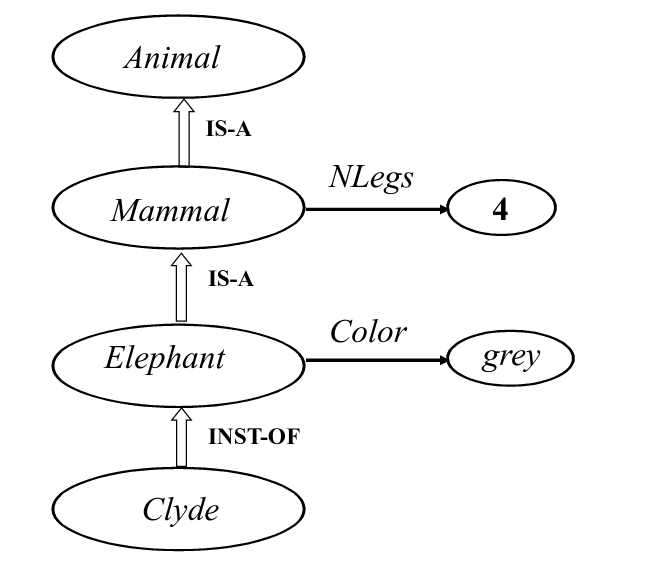
\includegraphics[width=\textwidth]{Images/inheritanceExample}
	\caption{Example of Inheritance in Semantic Network}
	\label{img:inheritance}
\end{figure}
The presence of exceptions does not create any problem, so we just take the most
specific information: the first that is found going up the hierarchy.\newline
Even if they can express n-ary predicates, semantic networks do not have the same
expressive power of FOL:
§ Existentials, $\lor$ and $\Rightarrow$ are not expressible or are expressible
only in special cases and this is not necessarily a bad thing since it suggests
a subset of FOL with interesting computational properties, explored in description logics.

A well -known example in AI are Sowa’s conceptual graphs, inspired by Pierce’s
existential graphs and they candidate as an intermediate schema for representing
natural language.\newline
Conceptual graphs, visible in figure \ref{img:conceptual}, rectangles are concepts
(possibly typed as in Person: John), circles are called conceptual relations:
the label is the name of the relation.

\begin{figure}
	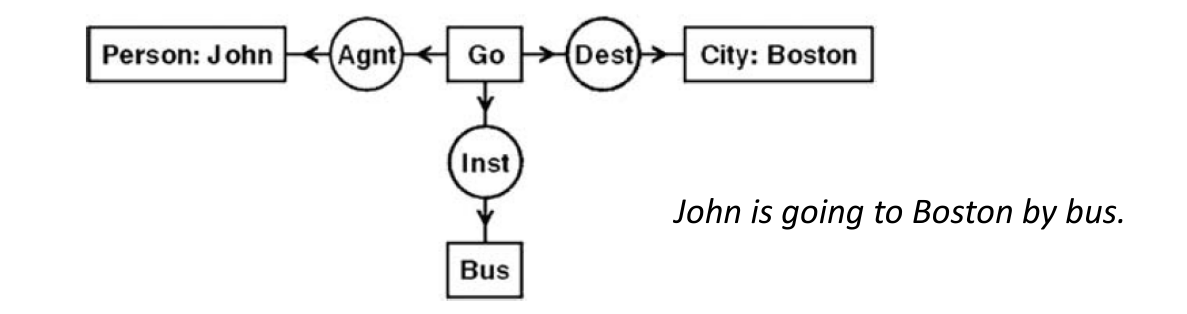
\includegraphics[width=\textwidth]{Images/conceptualGraph}
	\caption{Example of Conceptual graph}
	\label{img:conceptual}
\end{figure}

A more complex proposition, including implication, uses context boxes, so for example
“If a farmer owns a donkey, then he beats it” is represented in figure \ref{img:context}.

\begin{figure}
	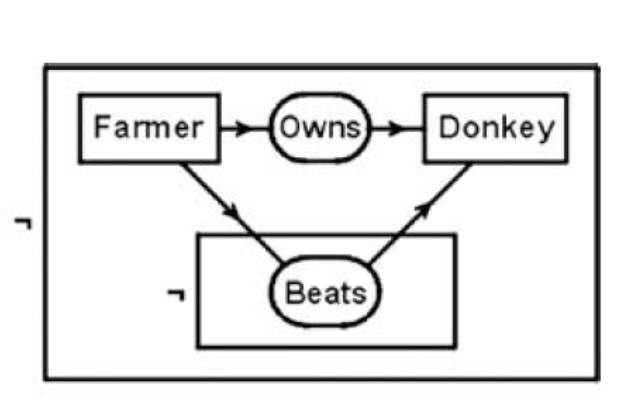
\includegraphics[width=\textwidth]{Images/complexConceptual}
	\caption{Complex example of Conceptual graph}
	\label{img:context}
\end{figure}
Woods and others point out the lack of “semantics” of semantic nets, so as a result
in the $80$’s KL-One introduces important ideas:
\begin{itemize}
   \item Concepts and roles (they are also nodes with a different status).
   \item Value restrictions ($v/r$)
   \item Numerical restrictions ($1$, NIL)
   \item A formal semantics
\end{itemize}
The double arrow is a IS-A relation and an example in figure \ref{img:klOne}.

\begin{figure}
	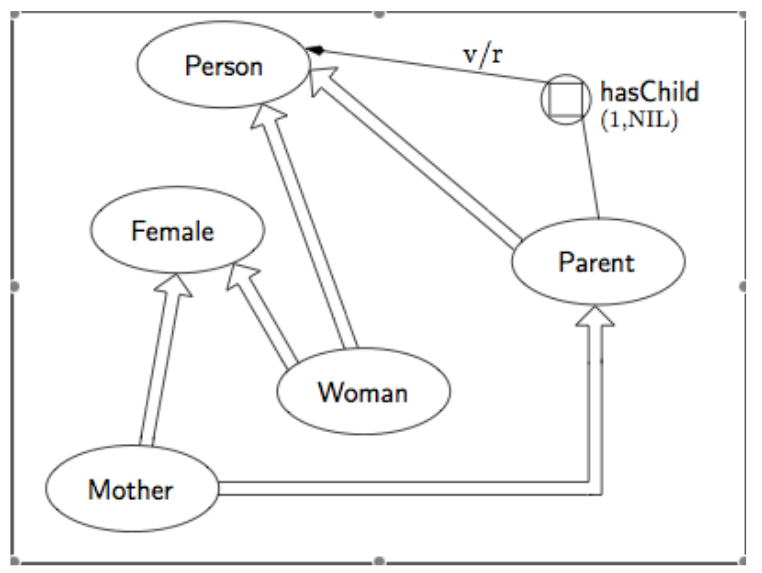
\includegraphics[width=\textwidth]{Images/klOne}
	\caption{Example of IS-A relation in KL One}
	\label{img:klOne}
\end{figure}
We may look at semantic networks as a convenient implementation for a part of
FOL and a representation and mechanism at the symbol level 
rather than at the knowledge level, with concepts defined in figure \ref{img:knowledgeConc}.

\begin{figure}
	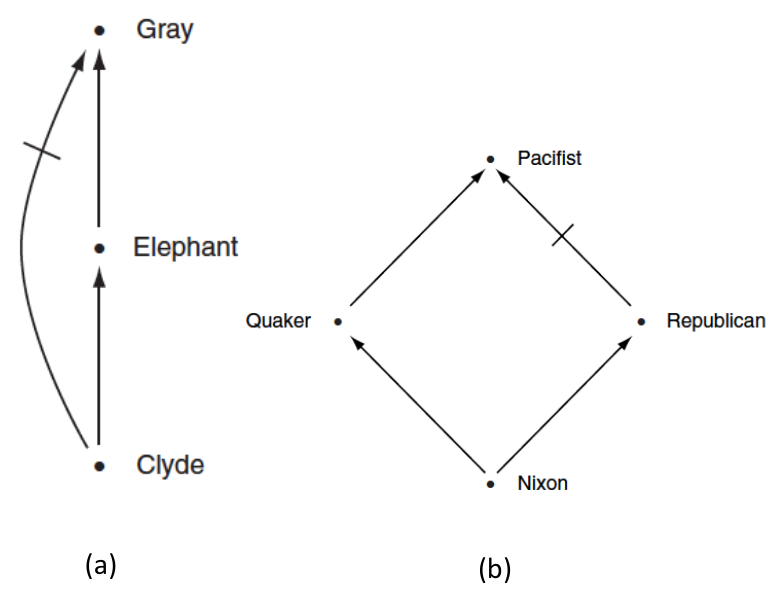
\includegraphics[width=\textwidth]{Images/knowledgeConc}
	\caption{Definition of representation done at the symbol level}
	\label{img:knowledgeConc}
\end{figure}
A more essential notation for inheritance networks are negated arcs, so more specific
information should win and there is also multiple inheritance, as we can see in figure
\ref{img:inheritanceNetwork}.

\begin{figure}
	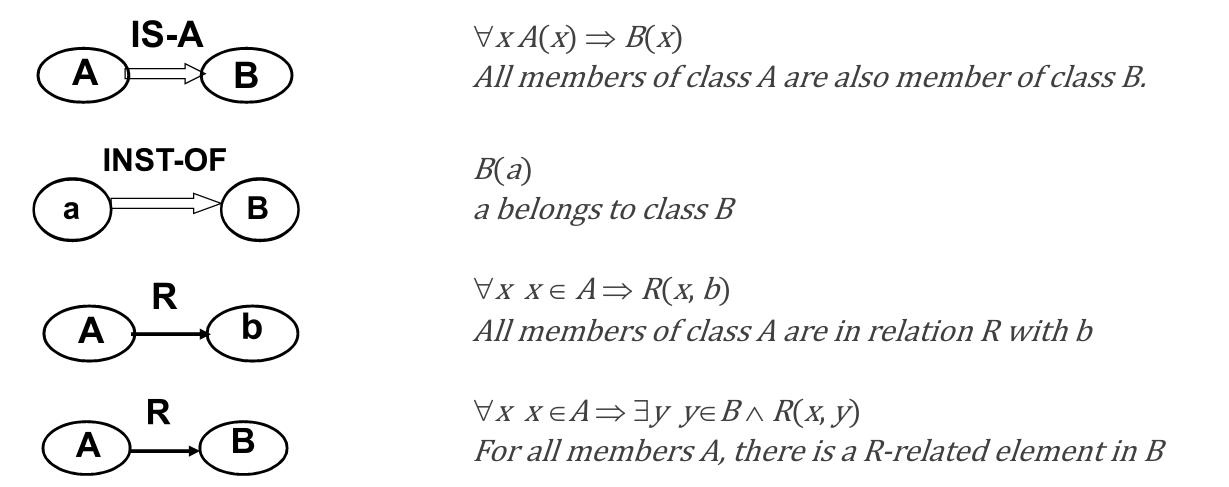
\includegraphics[width=\textwidth]{Images/inheritanceNetwork}
	\caption{Example of Inheritance Network}
	\label{img:inheritanceNetwork}
\end{figure}
Not so easy and there are two strategies:
\begin{itemize}
    \item Shortest path heuristics, based on minimal path length.
    \item Inferential distance, based on the topology (not path length).
\end{itemize}
The shortest path strategy fails in presence of redundant links such as $q$ (shortcuts),
as we can see in figure \ref{img:shortest} and the inferential distance strategy:
$A$ closer to $B$ than $C$ iff there is a path from a $A$ to $C$ through $B$.\newline
With shortest path it would conclude that Clyde is grey, instead inferential distance
it would conclude that Clyde is not grey.

\begin{figure}
	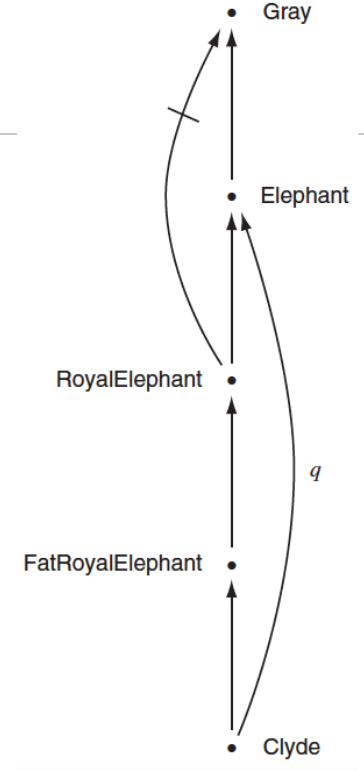
\includegraphics[width=\textwidth]{Images/shortestError}
	\caption{Example of shortest path failure with redundant links}
	\label{img:shortest}
\end{figure}

\emph{WordNet}, a big lexical resource organized as a Semantic network ($122.000$ terms),
names, verbs, adjectives, adverbs are organized in sets of synonims (synsets) which
are a representation of a concepts ($117.000$ synset); a syntactic word is associated
with a set of synsets: the word senses and uses of WordNet in computational linguistics are:
\begin{itemize} 
   \item Query expansion with synonyms or hyperonyms.
   \item Semantics distance among words.
   \item Word sense disambiguation.
   \item Semantic category of a word (or supersense).
\end{itemize}
The structure of WordNet is visible in figure \ref{img:wordnet}.

\begin{figure}
	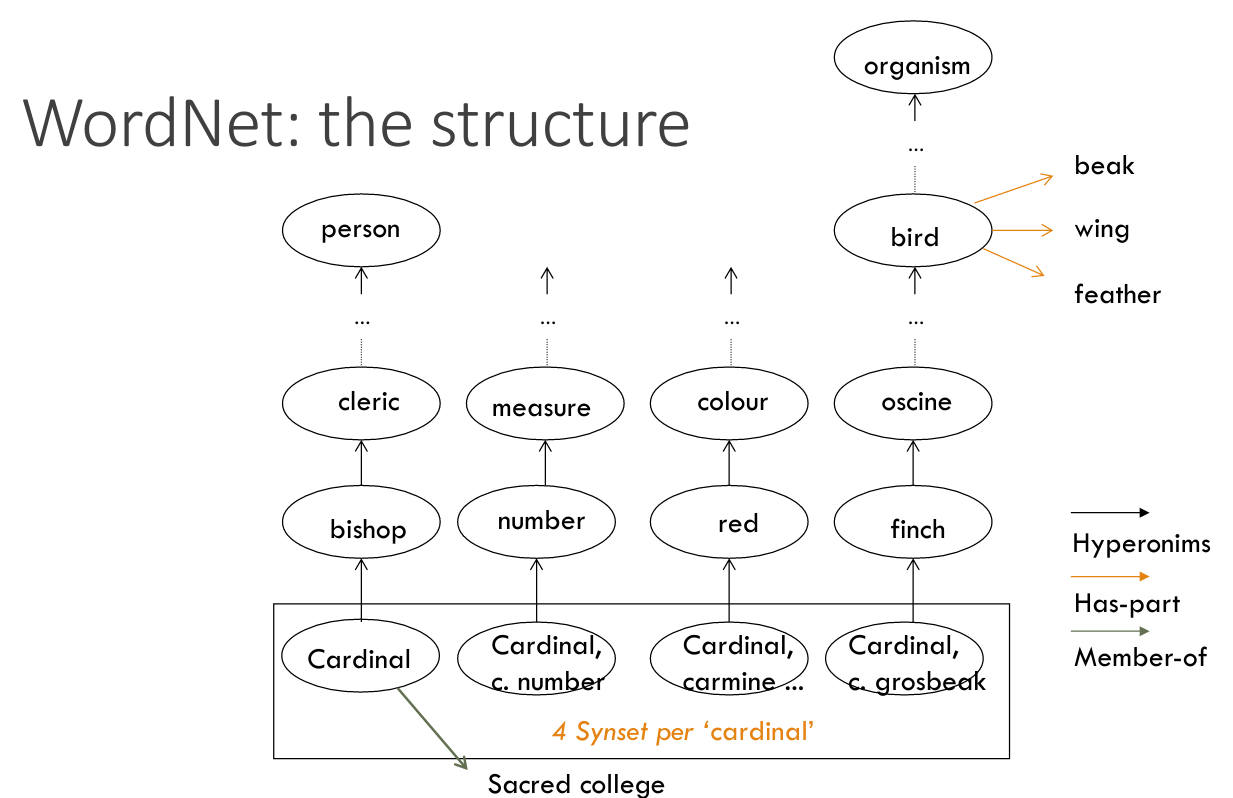
\includegraphics[width=\textwidth]{Images/wordnet}
	\caption{Structure of WordNet}
	\label{img:wordnet}
\end{figure}
\emph{Knowledge graphs} are large-scale knowledge bases have been built including:
\begin{description}
    \item [Open access: ] Dbpedia, WikiData, Freebase, YAGO.
    \item [Proprietary: ] Microsoft's Satori, Google's Knowledge Graph,
	                  Google’s Knowledge vault.
\end{description}
From $2012$ Google uses the knowledge graph with its search engine, structured data
coming from many sources, including the CIA World Factbook, Wikidata, Wikipedia, Freebase
and has more than $70$ billion facts in $2016$.\newline
Since $2014$, Google’s Knowledge Vault contains facts derived automatically from the
web with machine learning techniques and facts have an associated confidence value.

It is very natural to think of knowledge not as a flat collection of sentences, but
rather as structured and organized in terms of the objects the knowledge is about.\newline
Complex objects have attributes, parts constrained in various ways, objects might have
a behavior that is better expressed as procedures and this is very much
as in Object Oriented Programming.\newline
Marvin Minsky in $1975$ suggested the idea of using a structured representation
of objects, called frames, to recognize and deal with new situations.

Knowledge is organized in complex mental structures called \emph{frames}, and 
the essence of the theory is "When one encounters a new situation (or makes a 
substantial change in one's view of the present problem) one selects from memory
a structure called a frame.\newline
This is a remembered framework to be adapted to fit reality 
by changing details as necessary.".\newline
A frame is a data-structure for representing a stereotypical object or situation.

There are two types of frames:
\begin{description}
   \item [individual frames] used to represent single objects.
   \item [generic frames] used to represent categories or classes of objects.
\end{description}
An individual frame is a collection of slot-fillers pairs, and fillers can be:
\begin{itemize}
   \item values, usually default values.
   \item constraints on values.
   \item the names of other individual frames.
   \item the special slot INSTANCE-OF
\end{itemize}
Generic frames are similar and fillers can be the special slot IS-A or procedures 
like IF-ADDED, activated when the slot receives a value and IF-NEEDED,
activated when the value is requested.\newline
These procedures are called procedural attachments or demons, so the :INSTANCE-OF 
and :IS-A slots organize frames in frame systems.\newline
They have the special role of activating inheritance of properties and procedures.\newline
In frames, all values are understood as default values, which can be overridden and
example of frames are visible in figure \ref{img:frames}.\newline
Attached procedures provide a flexible, organized framework for computation and 
reasoning has a procedural flavor.\newline
A basic reasoning loop in a frame system has three steps:
\begin{description}
   \item [Recognition: ] a new object or situation is recognized as instance
	                 of a generic frame.
   \item [Inheritance: ] any slot fillers that are not provided explicitly but can be 
	                 inherited by the new frame instance are inherited.
   \item [Demons: ] for each slot with a filler, any inherited IF-ADDED procedure is run,
       possibly causing new slots to be filled, or new frames to be instantiated,
       until the system stabilizes, then the cycle repeats.
\end{description}
\begin{figure}
	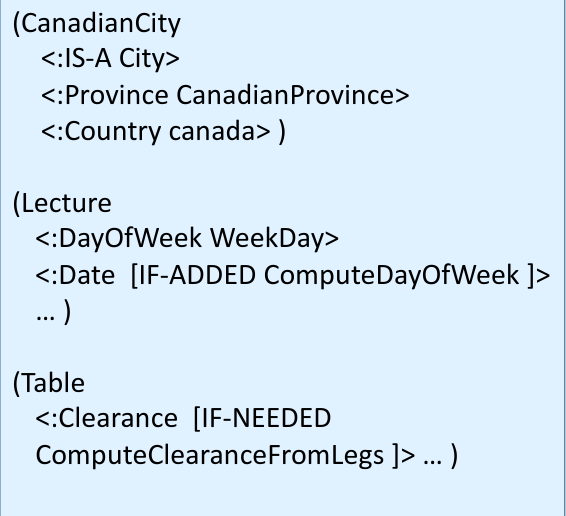
\includegraphics[width=\textwidth]{Images/frames}
	\caption{Example of Frames}
	\label{img:frames}
\end{figure}
When the filler of a slot is requested:
\begin{enumerate}
    \item if there is a value stored in the slot, the value is returned.
    \item otherwise, any inherited IF-NEEDED procedure is run to compute the filler
	  for the slot, and this may cause other slots to be filled, or new frames
	  to be instantiated.
\end{enumerate}
Frame-based representation languages and OOP systems were developed at the
same time, and they look similar and certainly one could implement 
a frame system with OOP.\newline
Important difference is that frame systems tend to work in a cycle:
\begin{itemize}
    \item Instantiate a frame and declare some slot fillers
    \item inherit values from more general frames
    \item trigger appropriate forward-chaining procedures
    \item when the system is quiescent, stop and wait for the next input
\end{itemize}
The designer can control the amount of "forward" reasoning that should be
done (in a data-directed fashion) or "backward" (in a goal-directed fashion).

Applications of frames are story understanding, Scene recognition in vision, tools
for building expert systems (possibly together with rules) and the idea of frames
was also used in building "FrameNet": a large NL resource based on the theory
of "frame-based" semantics.

\emph{FrameNet} is a resource consisting of collections of NL sentences syntactically and
semantically annotated, organized in frames.\newline
Frame semantics, the meaning of words emerges from the role they have in the 
conceptual structure of sentences and knowledge is structures in $16$ general domains:
time, space, communications, cognition, health and also has $6000$ Lexical elements,
and $130.000$ annotated sentences; 
an example in FrameNet is visible in figure \ref{img:framenet}.

\begin{figure}
	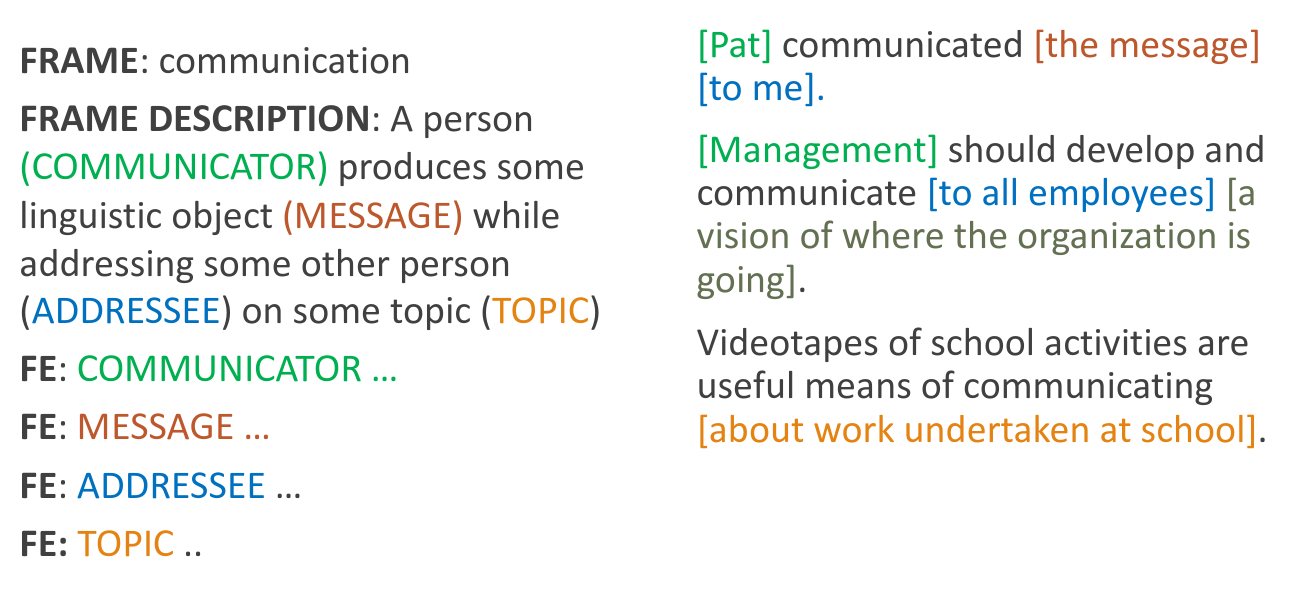
\includegraphics[width=\textwidth]{Images/framenet}
	\caption{Example of FrameNet}
	\label{img:framenet}
\end{figure}

\section{Description Logics}
Most of the reasoning takes place at the level of categories rather than on individuals,
so if we organize knowledge in categories and subcategories (in a hierarchy) it is enough
to classify an object, according to its perceived properties, in order to infer 
properties of the categories to which it belongs.\newline
Inheritance is a common form of inference, which exploits structure and also 
ontologies will play a crucial role, providing a source of shared and precisely defined
terms that can be used in meta-data of digital objects and real world objects.

In the $80$'s we assist to a formalization of the ideas coming from semantic
networks and frames resulting in specialized logics.\newline
These logics, called terminological logics and later description logics find an
important application in describing “domain ontologies” and represent the
theoretical foundations for adding reasoning capabilities to the Semantic web.\newline
\emph{Ontology} is a formal model of an application domain (a conceptualization) and
subclass relations are important in defining the terminology and serve to
organize knowledge in hierarchical taxonomies (shared ontologies are the basis
for the semantic web).

The \emph{Semantic Web} is the vision of Tim Berners-Lee ($1998$) to gradually
develop alongside the “syntactic web” (or web of documents), for communication among people,
a “semantic web” (or web of data) for communication among machines.\newline
The semantic web is a huge distributed network of linked data which can be used by programs
as well, provided their semantics is shared and made clear 
(this is the role of formal ontologies).\newline
These data comply with standard web technologies: Unicode encoding, XML, URI,
HTTP web protocol.

The technologies used in Semantic Web, visible in \ref{img:semantic}, are the following:
\begin{itemize}
   \item Unicode and URI (Universal Resource Identifier)
   \item XML for syntactic interoperability
   \item RDF (Resource Description Framework) is a language to describe binary
         relations between resources (subject, predicate, object).
   \item RDF schema (RDFS) used to define classes, relations between classes,
	 to constrain domains and co-domains of relations and this is basic language
	 for ontologies.
   \item OWL is the web ontology language, one among many description logics
         elected as standard by the W3C.
\end{itemize}
\begin{figure}
	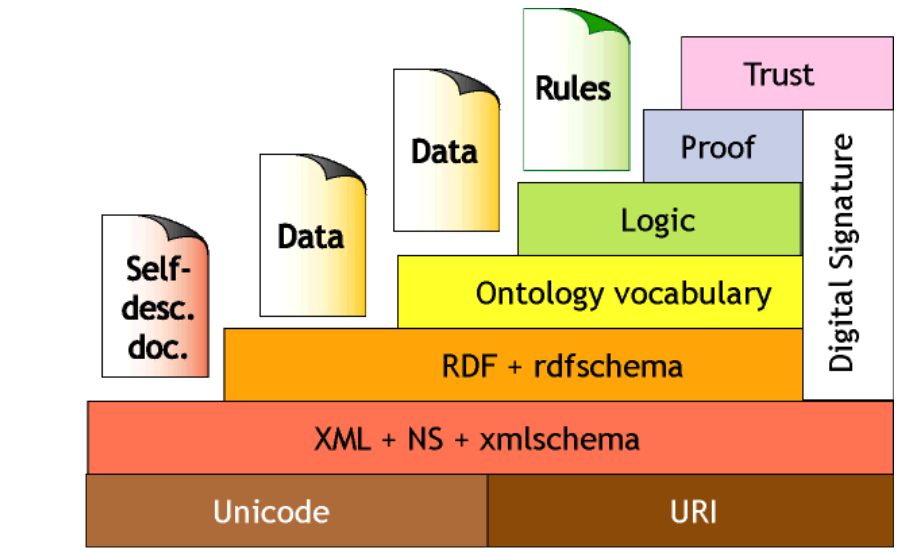
\includegraphics[width=\textwidth]{Images/semanticTechnologies}
	\caption{Technologies used in Semantic Web}
	\label{img:semantic}
\end{figure}
\emph{Description logics} can be be seen as:
\begin{enumerate}
   \item Logical counterparts of network knowledge representation schema, frames
         and semantic networks; in this formalization effort, defaults and exceptions
	 are abandoned and the ideas and terminology (concept, roles, inheritance
	 hierarchies) are very similar (to KLOne in particular).
   \item Contractions of first order logic (FOL), investigated to obtain better
         computational properties and attention to computational complexity/decidability
	 of the inference mechanisms.
\end{enumerate}
Each DL is characterized by operators for the construction of terms, that are of $3$ types:
\begin{description}
    \item [Concepts: ] corresponding to unary relations, with operators for the construction
	   of complex concepts: and($\cap$), or($\cup$), not($\neg$), all($\forall$), 
	   some ($\exists$), atleast ($\geq n$), almost ($\leq n$) and so on.
    \item [Roles: ] corresponding to binary relations, possibly together with operators
	            for construction of complex roles.
    \item [Individuals:]  only used in assertions.
\end{description}
Assertions are kept separate and can be only of two types:
\begin{itemize}
   \item $i: C$, where $i$ an individual and $C$ is a concept.
   \item $(i, j): R$, where $i$ and $j$ are individual and $R$ is a role.
\end{itemize}
In figure \ref{img:kbDescription} is possible to note an example of KB based on 
description logic and we define the logic $AL$ as the syntax of terms 
in figure \ref{img:logicAL}.

\begin{figure}
	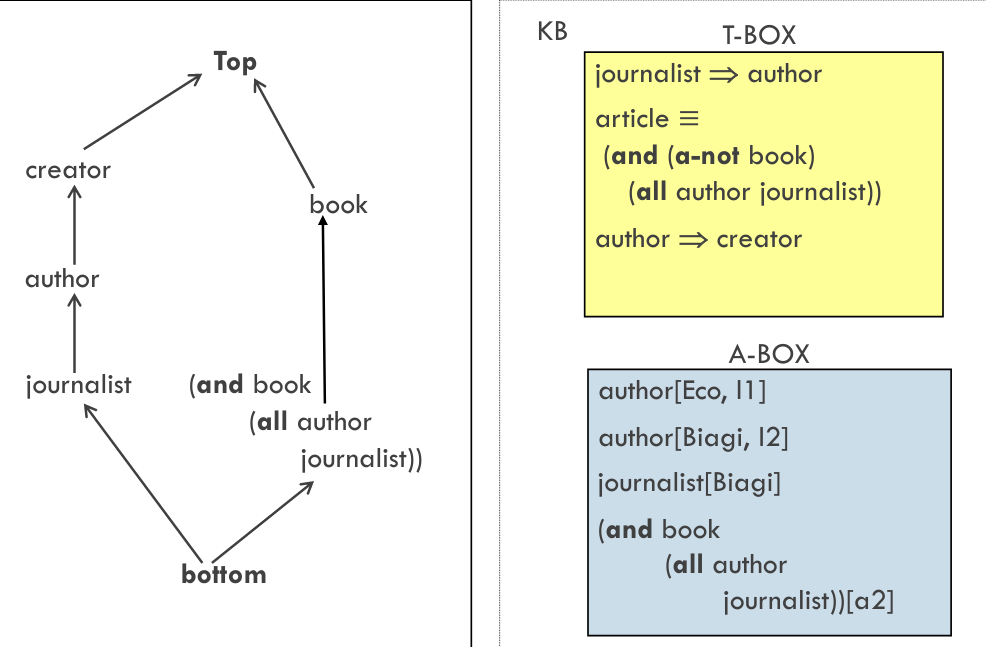
\includegraphics[width=\textwidth]{Images/exampleKB}
	\caption{Example of KB Description}
	\label{img:kbDescription}
\end{figure}
\begin{figure}
	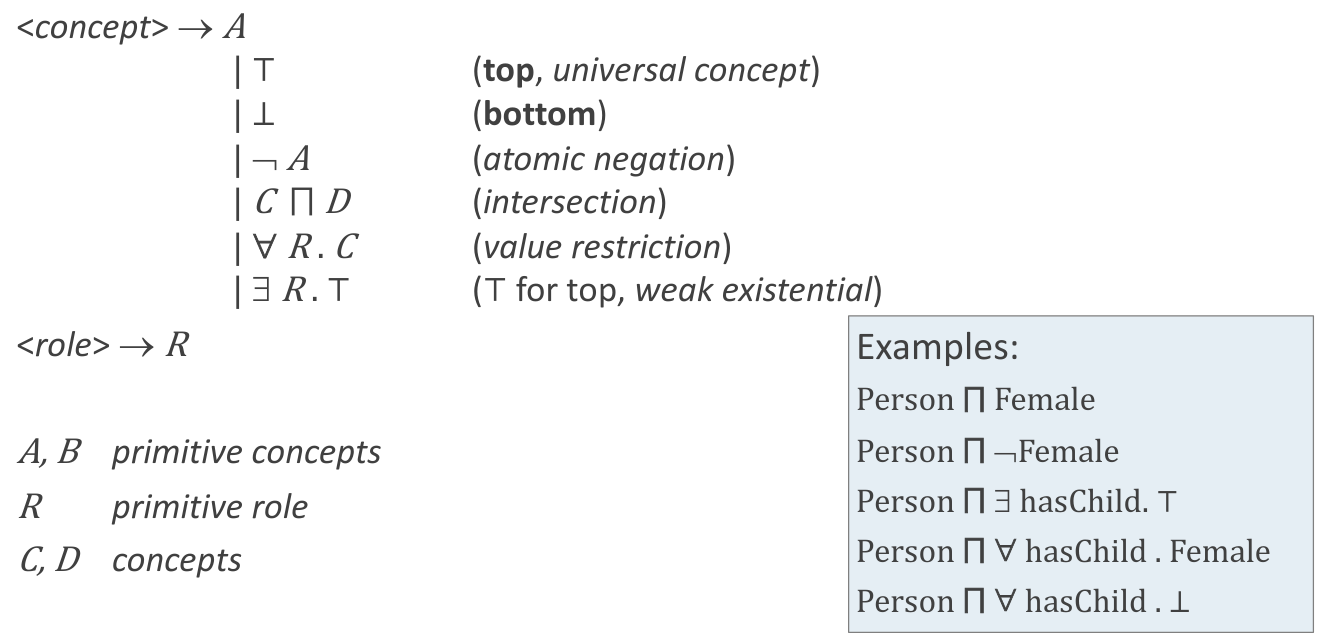
\includegraphics[width=\textwidth]{Images/logicAL}
	\caption{Definition of syntax of Logic $AL$}
	\label{img:logicAL}
\end{figure}
The semantics of $AL$ consist of $\Delta^I$, interpretation domain (a set of individuals) 
and $I$ an interpretation function which assign for atomic concepts 
$A: A^I \subseteq \Delta^I$, for atomic roles $R: R^I \subseteq \Delta^I \times \Delta^I$
and for individual constants $a: a^I \in \Delta^I$.\newline
We have some rules visible in figure \ref{img:semanticAL} and we have also $4$ 
more expressive logics, defined as:
\begin{description}
   \item [$U$ union: ] $(C \cup D)^I = (C^I \cup D^I)$ 
   \item [$E$ full existential: ] ($\exists R.C)^I = \{ a \in \Delta^I : \exists b. (a, b)
	                          \in R^I \cap b \in C^I \}$
   \item [$N$ numerical restrictions: ] 
	   \[ (\geq n R)^I = \{ a \in \Delta^I : |\{b : (a, b) \in R^I\}| \geq n\} \]
	   \[ (\leq n R)^I = \{ a \in \Delta^I : |\{b : (a, b) \in R^I\}| \leq n\} \]
   \item [$C$ full complement: ] $(\not C)^I = \Delta ^ I - C^I$
\end{description}
\begin{figure}
	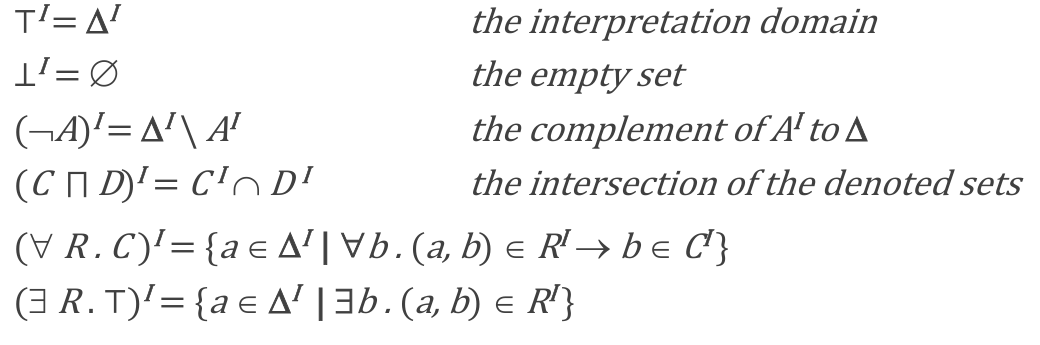
\includegraphics[width=\textwidth]{Images/rulesAL}
	\caption{Some rules for logic $AL$}
	\label{img:semanticAL}
\end{figure}
Different description logics are obtained by adding other constructors to AL and 
we obtain the lattice visible in figure \ref{img:ALLattice}, where not all of them 
are distinct so for example $ALUE = ALC$.

\begin{figure}
	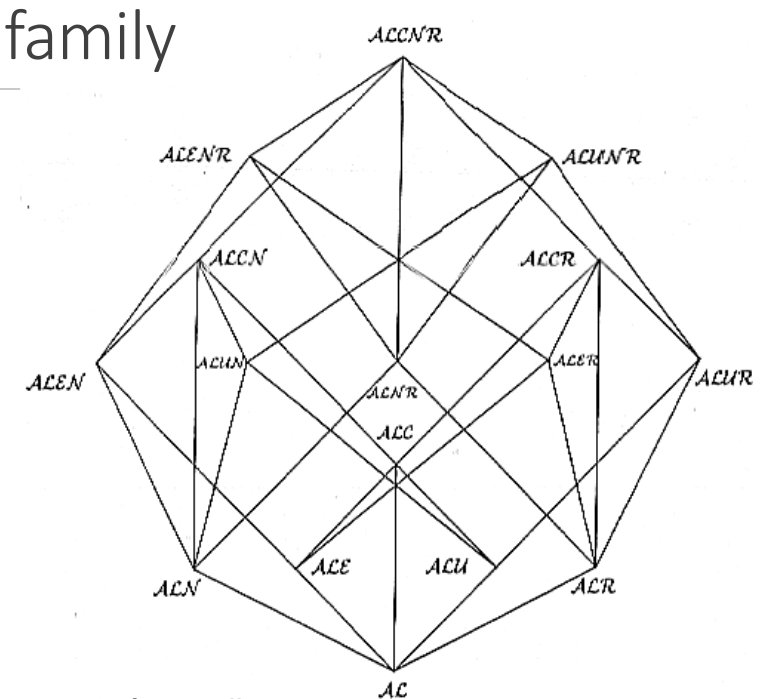
\includegraphics[width=\textwidth]{Images/ALLattice}
	\caption{Lattice of $AL$ logics}
	\label{img:ALLattice}
\end{figure}
We have the terminological axioms $T$ defined as:
\[ C \subseteq D \text{ inclusion of concepts } C^I \subseteq D^I \]
\[ R \subseteq S \text{ inclusion of roles } R^I \subseteq S^I \]
\[ C \equiv D \text{ equality of concepts } C^I \equiv D^I \]
\[ R \equiv S \text{ equality of roles } R^I \equiv S^I \]
We have that equalities introduce a symbol on the left and we have a \emph{terminology},
when symbols appear on the left not more than once; we have a \emph{primitive symbols} in
case appear only on the right and a \emph{defined symbols} if appear also on the left.

If a terminology is acyclic, an example is visible in figure \ref{img:acyclicTerm}, it can
be expanded by substituting to defined symbols their definitions.\newline
In the case of acyclic terminologies the process converges and the expansion $T^e$ is unique.

\begin{figure}
	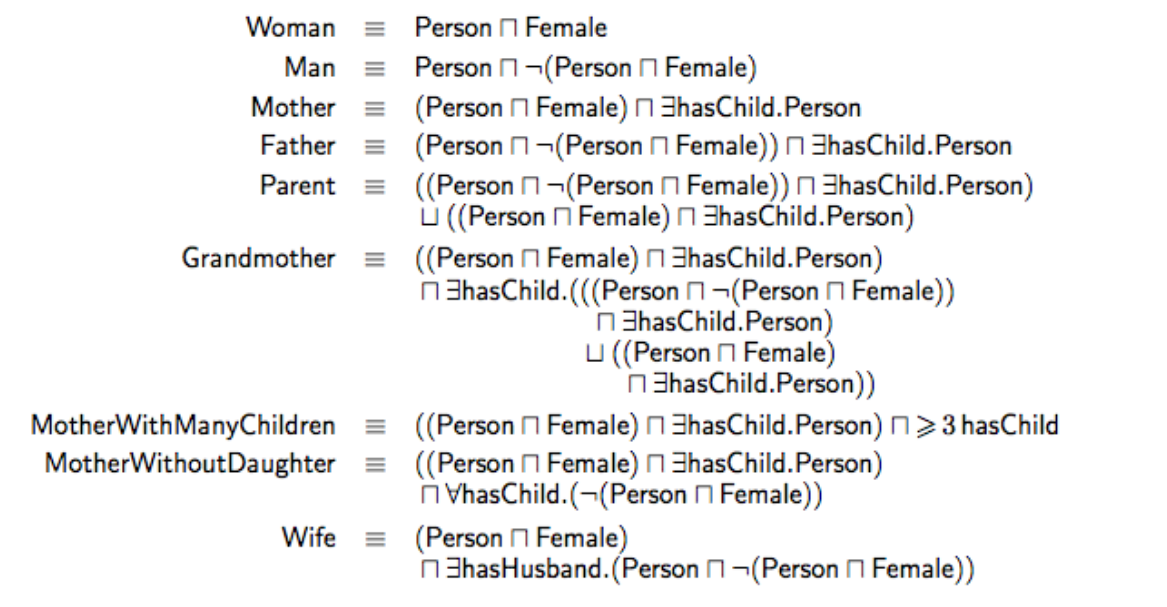
\includegraphics[width=\textwidth]{Images/acyclic}
	\caption{Example of Acyclic description logics}
	\label{img:acyclicTerm}
\end{figure}
Properties of $T^e$ are the following:
\begin{itemize}
   \item In $T^e$ each equality has the form $C \equiv D^e$ where $D^e$ contains only 
	 primitive symbols.
   \item $T^e$ contains the same primitive and defined symbols of $T$
   \item $T^e$ is equivalent to $T$.
\end{itemize}
An example of expansion is visible in figure \ref{img:expandedTerminology} and inclusion
axioms are called \emph{specializations}, like for example $Woman \subseteq Person$.\newline
A \emph{generalized terminolohy}, with inclusion axioms, if acyclic, can be transformed in 
an equivalent terminology with just equivalence axioms
\[ A \subseteq C \to A \equiv A' \cap C \]
where $A'$ is a new primitive symbol.\newline
This also means that specializations do not add expressive power to the language, 
at least in the case of acyclic terminologies.

\begin{figure}
	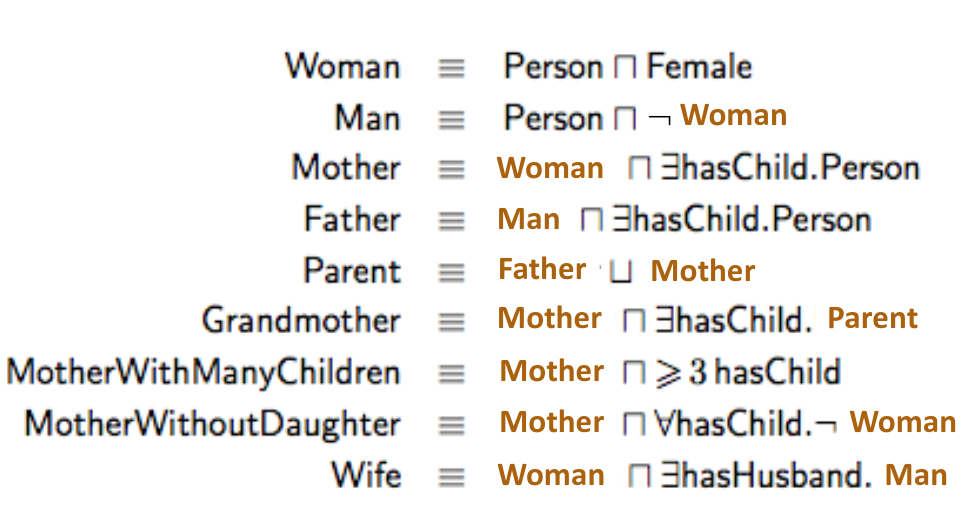
\includegraphics[width=\textwidth]{Images/expanded}
	\caption{Example of an expansion of terminology}
	\label{img:expandedTerminology}
\end{figure}
An A-BOX is a set of assertions of the following type $a: C$ assertion over concepts
(meaning $a^I \in C^I$) and $(b, c) : R$ assertions over roles (meaning $(b^I, c^I) \in R^I$,
where $a, b, c, d, \dots$ are individuals.\newline
In description logic we make an assumption that different indivudal constants refer to
different individuals, and that is called \emph{Unique Name Assumption} (UNA).

It is always possible to translate DL assertions into FOL, so we define a translation
function $t(C, x)$ which returns a FOL formula with $x$ free
\[ t(C, x) \to C(x) \]
In figure \ref{img:assertTranslation} we have translation rules for assertions and 
in figure \ref{img:termTranslatin} we have translation rules for terms.

\begin{figure}
	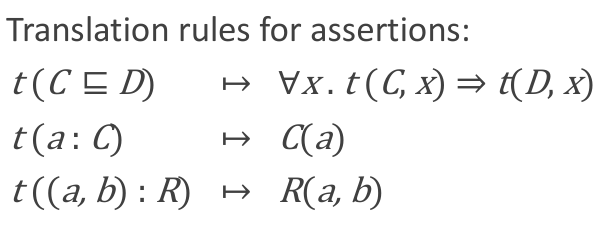
\includegraphics[width=\textwidth]{Images/assertTranslation}
	\caption{Translation rules for assertions}
	\label{img:assertTranslation}
\end{figure}

\begin{figure}
	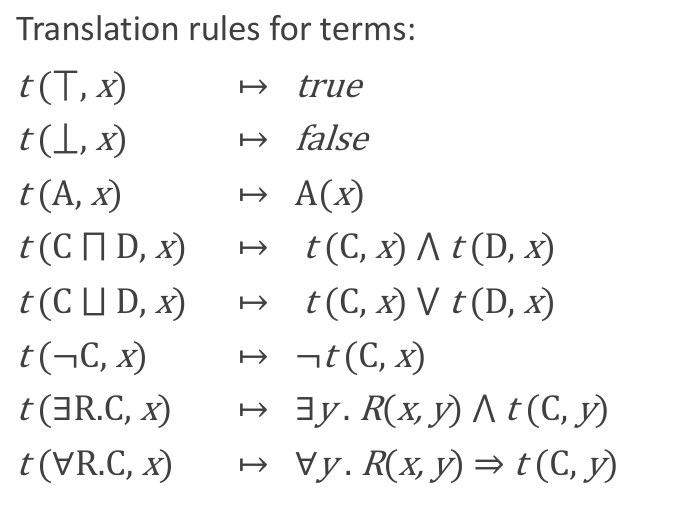
\includegraphics[width=\textwidth]{Images/termTranslation}
	\caption{Translation rules for terms}
	\label{img:termTranslatin}
\end{figure}
We have that the knowledge base in description logics is defined by $K = (T, A)$, where
$T$ is the T-BOX terminological component and $A$ is the A-BOX the assertional component.

An interpretation $I$ satisfies $A$ and $T$ (therefore $K$) iff it satisfies 
any assertion in $A$ and definition in $T$ ($I$ is a model of $K$).\newline

Classical decision problems in DL are the following:
\begin{description}
   \item [Satisfiability of a KB:]  $KBS(K)$ answer if there is a model for $K = (T, A)$.
   \item [Logical consequence of a KB: ] $K \models a:C$ also called instance checking.
   \item [Concept satisfiability $CS(c)$:] estabilish if is there an interpretation
	   different from the empty set.
   \item [Subsumption: ] $K \models C \subseteq D$ if for every model $I$ di $T$,
	   $C^I \subseteq D^I$.
   \item [Concept equivalence:] $K \models C \equiv D$.
   \item [Disjointness: ] answer if $C^I \cap D^I = \emptyset$ for any model $I$ of $T$.
   \item [Retrieval: ] find all individuals which are instances of $C$.
   \item [Most Specific Concept (MSC): ] given a set of individuals, find the most
	  specific concept of which they are instances and this is used for classification.
   \item [Least Common Subsumer (LCS): ] given a set of concepts, find the most specific
	 concept which subsumes all of them and is also used for classification.
\end{description}
Decision problems are not independent, infact all problems can be reduced to $KB$ 
satisfiability, so we have for esample that concept consistency is satisfied iff 
$K \cup \{a:C\}$ is satisfiable, instance checking $K \models a:C$ iff $K \cup \{a:\neg C\}$
is unsatisfiable; this is for some aspect reconduble to classic logic deduction.

The most used method is a technique for verifying satisfiability of a KB (KBS), and it is
a variant of a method for natural deduction, called \emph{semantic tableaux}
(It applies constraint propagation).\newline
Basic idea is that each formula in $KB$ is a constraint on possible interpretations and 
complex constraints are decomposed in simpler constraints by means of propagation rules
until we obtain, in a finite number of steps, atomicvconstraints,
which cannot further decomposed.\newline
If the set of atomic constraints contains an evident contradiction then the KB is
not satisfiable, otherwise a model has been found and this technique is simple,
modular, useful for evaluating complexity of decision algorithm.

Preliminary steps before $KBS$ are the following:
\begin{description}
   \item [Terminology expansion: ] a preliminary step consisting in resolving 
	   specializations, getting rid of the terminology by substituting defined
           concepts in $A$ with their definitions.
   \item [Normalization: ] assertions are transformed in negation normal form,
	   by applying the following rules until every occurrence of
           negation is in front of a primitive concept.\newline
	   These transformed assertions constitute the initial set of constraints
	   for the $KBS$ algorithm.
\end{description}
A constraint is an assertion of the form $a:C$ or $(b, c):R$ where $a,b$ and $c$ are
constants (distinct individuals) or variables $(x, y, \dots)$ referring to individuals but
not necessarily distinct ones.\newline
A constraint set $A$ is satisfiable iff there exists an interpretation satisfying all the
constraints in A and each step of the algorithm decomposes a constraint into a simpler one
until we get a set of elementary constraints, or a contradiction (clash) is found.\newline
For ALC a clash is one of the following types $\{a:C, a:\neg C\}$ or $\{a: \perp\}$.

\emph{Completion forest} are data structures for supporting the execution of the algorithm,
where for each individual $a$ appearing in assertions in $A$, a labelled tree is initialized.

The label is a set of the constraints that apply to $a$, so if $A$ contains $a:C$,
we add the constraint $C$ to the label of $a$, or if $A$ contains $(a, b):R$,
we create a successor node of $a$ for $b$ to represent the $R$ relation between them.

\begin{figure}
	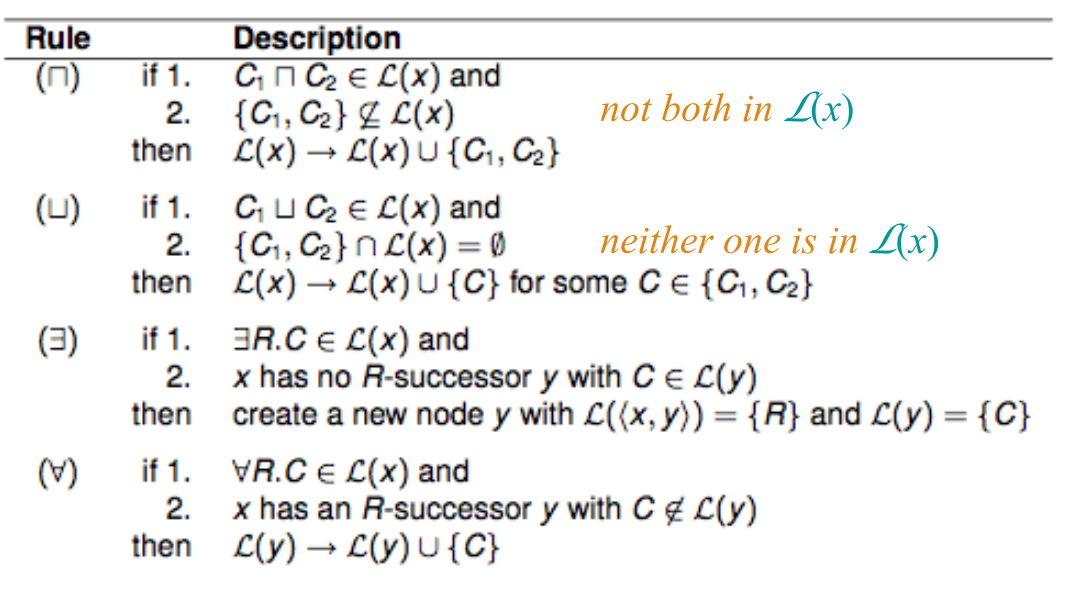
\includegraphics[width=\textwidth]{Images/rulesPropagation}
	\caption{Rules for constraint propagation}
	\label{img:rulesPropagation}
\end{figure}
In figure \ref{img:rulesPropagation} we have the rules for constraint propagation and also
most rules are deterministic, but the rule for disjunction is non deterministic: 
its application results in alternative constraints sets, so we have a fork in the proof.

$A$ is satisfiable iff at least one of the resulting constraint set is satisfiable, and 
$A$ is unsatisfiable iff all the alternatives end up with a clash.

The result is invariant with respect to the order of application of the rules, and we have
the following result for correctness and completeness:
\begin{description}
   \item [Correctness: ] if the algorithm terminates with at least one primitive constraint
	   set and no clashes, then $A$ is satisfiable and from the constraints
           we can derive a model.
   \item [Completeness: ] if a knoweldge base $A$ is satisfiable, then the algorithm
                          terminates producing at least a finite model without clashes.
\end{description}
We have $KBS$ decidable for $ALC$ and also for $ALCN$.

\begin{figure}
	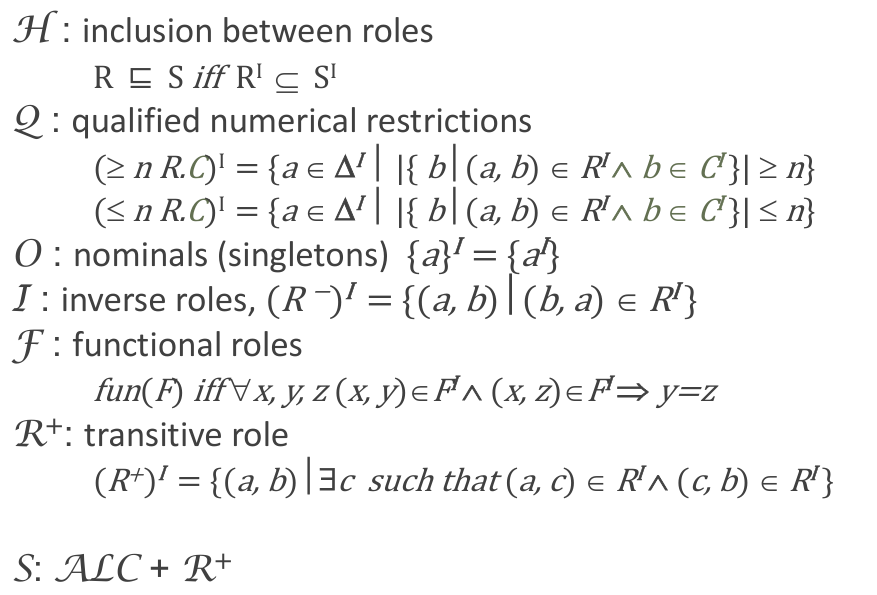
\includegraphics[width=\textwidth]{Images/addConstructors}
	\caption{Additional constructors to description logics}
	\label{img:addConstructors}
\end{figure}
In figure \ref{img:addConstructors} is possible to note possible additional constructors to
description logics, ans we have that \emph{OWL-DL} is equivalent to $SHOIN$, instead
\emph{OWL-Lite} is equivalent to $SHIF$; these two language are the ontology language
for Semantic Web.

\begin{figure}
	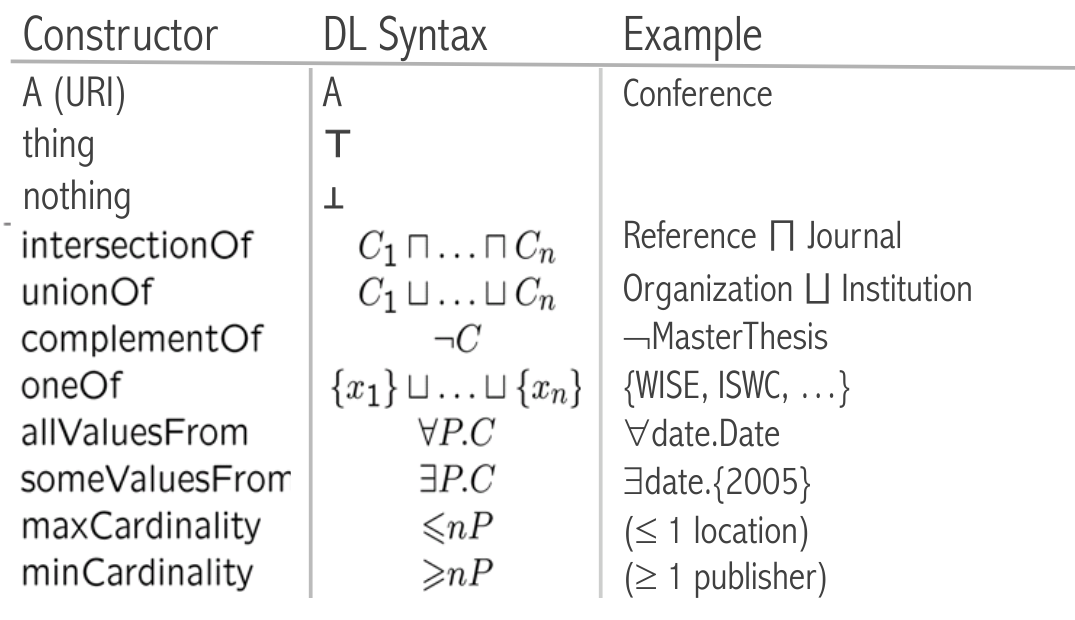
\includegraphics[width=\textwidth]{Images/owlSyntax}
	\caption{Syntax for OWL}
	\label{img:owlSyntax}
\end{figure}

\begin{figure}
	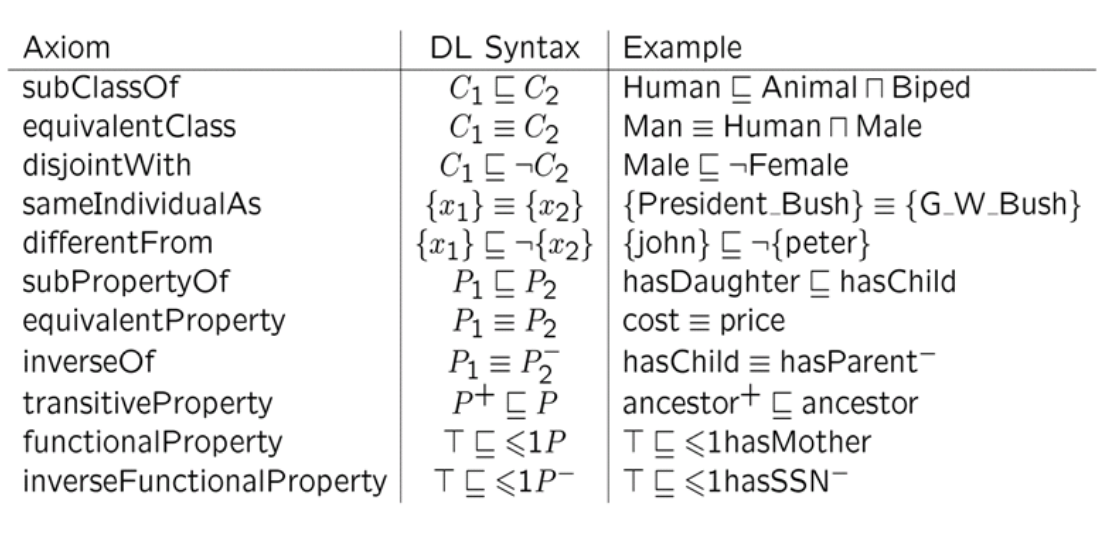
\includegraphics[width=\textwidth]{Images/owlAxioms}
	\caption{Axioms defined for OWL}
	\label{img:owlAxioms}
\end{figure}
The syntax for OWL is defined by figure \ref{img:owlSyntax}, axioms by figure 
\ref{img:owlAxioms}, the XML syntax used in visible in figure \ref{img:owlXML} and in the
end in figure \ref{img:DLresults} is possible to see complexity and decitability results
for DL's.

\begin{figure}
	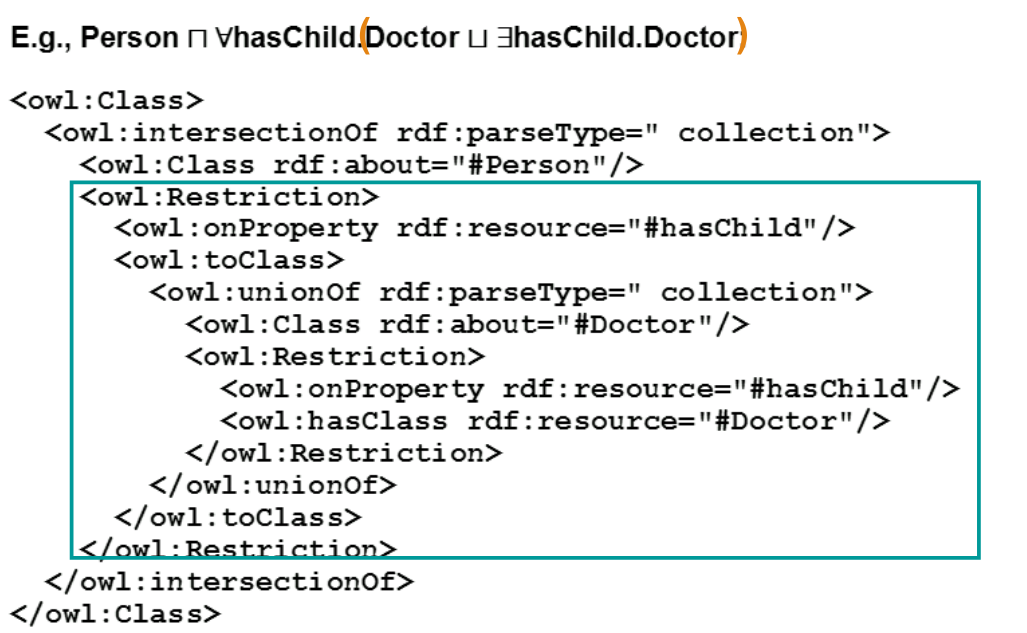
\includegraphics[width=\textwidth]{Images/owlXML}
	\caption{XML syntax used for OWL}
	\label{img:owlXML}
\end{figure}
\begin{figure}
	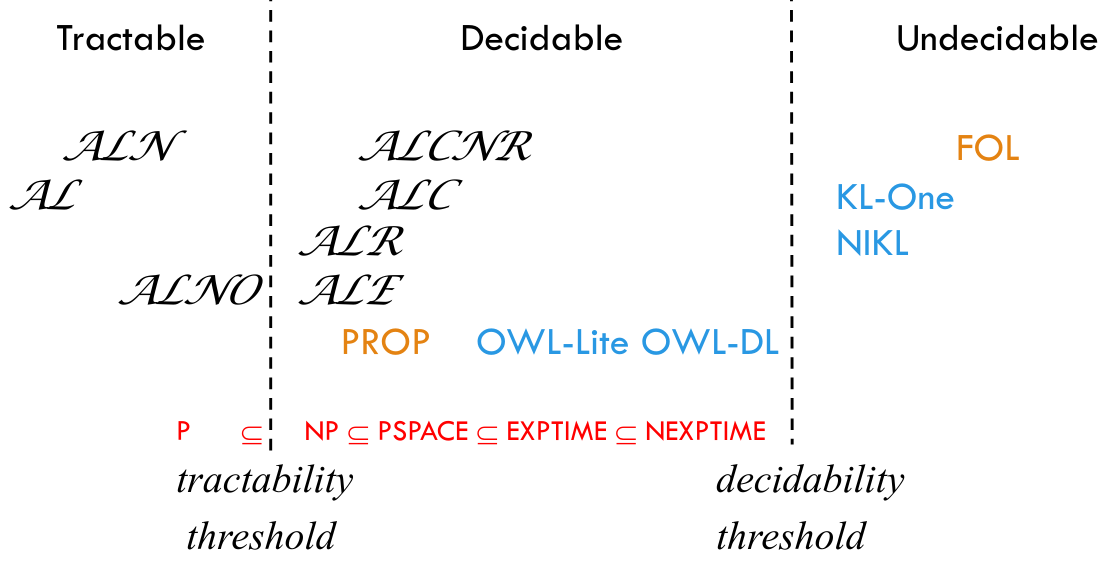
\includegraphics[width=\textwidth]{Images/DLresults}
	\caption{Complexity and decidability results for DL}
	\label{img:DLresults}
\end{figure}

